\documentclass[12pt]{article}
\usepackage{amsmath}
\usepackage{amsthm}
\usepackage{amssymb}
\usepackage{euscript}
\usepackage{mathrsfs}
\usepackage{bm}
\usepackage{enumitem}
\usepackage{tikz}
\usepackage{mathtools}
\usepackage{float}
\usepackage{hyperref}
\usepackage{boldline}
\usepackage{indentfirst}
\usepackage{environ}
\usepackage{courier}
\usetikzlibrary{positioning}

\renewcommand{\labelitemii}{$\vartriangleright$}
\renewcommand{\labelitemiv}{$\Join$}

\makeatletter
\newsavebox{\measure@tikzpicture}
\NewEnviron{scaletikzpicturetowidth}[1]{%
  \def\tikz@width{#1}%
  \def\tikzscale{1}\begin{lrbox}{\measure@tikzpicture}%
  \BODY
  \end{lrbox}%
  \pgfmathparse{#1/\wd\measure@tikzpicture}%
  \edef\tikzscale{\pgfmathresult}%
  \BODY
}
\makeatother

\numberwithin{equation}{section}

\hypersetup{
    colorlinks=true,
    % linkcolor=blue,
    linkcolor=[RGB]{0,0,128},
    % filecolor=[RGB]{0,0,128},
    filecolor=magenta,
    urlcolor=cyan,
    citecolor = [RGB]{128,0,128}
}

\newcommand{\myref}[2]{\hyperref[#2]{#1 \ref*{#2}}}
\newcommand{\myrefT}[1]{\hyperref[#1]{Theorem \ref*{#1}}}
\newcommand{\myrefP}[1]{\hyperref[#1]{Proposition \ref*{#1}}}
\newcommand{\myrefL}[1]{\hyperref[#1]{Lemma \ref*{#1}}}
\newcommand{\myrefD}[1]{\hyperref[#1]{Definition \ref*{#1}}}
\newcommand{\myrefn}[3]{\hyperref[#2]{#1 \ref*{#2} (#3)}}

% \input{dynkinMacros.tex}
% \input{dynkinEMacros.tex}
% \renewcommand{\qedsymbol}{}
\newcommand{\ssm}{\smallsetminus}

\newcommand{\para}[1]{\noindent\underline{#1}.}

\newcommand{\ti}{$\tau\textnormal{-invariant}$}
\newcommand{\prim}{\textnormal{Prim}_{\lambda}(\textnormal{U}(\gf))}

\newcommand{\ve}{\varepsilon}
\newcommand{\veo}{\varepsilon_1}
\newcommand{\vet}{\varepsilon_2}
\newcommand{\vei}{\varepsilon_i}
\newcommand{\vp}{\varphi}

% \newcommand{\inr}{\textnormal{In}^R}
% \newcommand{\inl}{\textnormal{In}^L}
% \newcommand{\inc}{\textnormal{In}}
% \renewcommand{\sc}{\textnormal{SC}}
% \newcommand{\re}{\textnormal{Re}}

\newcommand{\ag}{\alpha}
\newcommand{\bg}{\beta}
\newcommand{\g}{\gamma}
\newcommand{\dg}{\delta}
\newcommand{\rg}{\rho}
\newcommand{\kg}{\kappa}
\newcommand{\sg}{\sigma}
\newcommand{\tg}{\tau}
\renewcommand{\lg}{\lambda}

\renewcommand{\gg}{$\gamma \ $}
\newcommand{\ga}{$\alpha \ $}
\newcommand{\gt}{$\tau $}
\renewcommand{\(}{(\gamma)}
\newcommand{\atg}{\tilde\alpha}
\newcommand{\ags}[1]{{\ag_{#1}}}
\newcommand{\ao}{{\ag_1'}}

\newcommand{\gf}{\mathfrak g}
\newcommand{\hf}{\mathfrak h}

% needs a new name
%\newcommand{\th}[1]{{$\text{\it #1 }^{\underline{\textnormal{th}}}$}}
\renewcommand{\sf}{\mathscr F}
\newcommand{\dsf}{$\sf$}
\newcommand{\st}{\mathscr T}
% needs a new name  -- ok?
\newcommand{\so}[1]{\mathscr #1}


\newcommand{\snn}{{\mathscr S(n,n)}}
\newcommand{\smm}{{\mathscr S(M^L,M^R)}}
\renewcommand{\tan}{\mathscr T_A(n)}
\newcommand{\tn}{\mathscr T(n)}
\newcommand{\dtn}{$\tn$}
\newcommand{\tm}{\mathscr T(M)}
\newcommand{\dtm}{$\tm$}
\newcommand{\tcsn}{\mathscr T_C^S(n)}
\newcommand{\tbsn}{\mathscr T_B^S(n)}
\newcommand{\tsn}[1]{\mathscr T_#1(n)}
\newcommand{\tsm}[1]{\mathscr T_#1(M)}
\newcommand{\tnn}{\mathscr T(n,n)}
\newcommand{\tmm}{\mathscr T(M^L,M^R)}
\newcommand{\tkmm}{\mathscr T_K(M^L,M^R)}
\newcommand{\tsnn}[1]{\mathscr T_#1(n,n)}
\newcommand{\tsmm}[1]{\mathscr T_#1(M^L,M^R)}
\newcommand{\tdnn}{\mathscr T_D(n,n)}
\newcommand{\tdmm}{\mathscr T_D(M^L,M^R)}
\newcommand{\tdn}{\mathscr T_D(n)}
\newcommand{\tdm}{\mathscr T_D(M)}
\newcommand{\tcnn}{\mathscr T_C(n,n)}
\newcommand{\tcmm}{\mathscr T_C(M^L,M^R)}
\newcommand{\tcn}{\mathscr T_C(n)}
\newcommand{\tcm}{\mathscr T_C(M)}
\newcommand{\cm}{\mathscr C(M)}
\newcommand{\dm}{\mathscr D(M)}

\newcommand{\snnp}{\mathscr S'(n,n)}
\newcommand{\smmp}{\mathscr S'(M^L,M^R)}
\newcommand{\snnpp}{\mathscr S''(n,n)}
\newcommand{\smmpp}{\mathscr S''(M^L,M^R)}
\newcommand{\tnnp}{\mathscr T'(n,n)}
\newcommand{\tmmp}{\mathscr T'(M^L,M^R)}
\newcommand{\tnnpp}{\mathscr T''(n,n)}
\newcommand{\tmmpp}{\mathscr T''(M^L,M^R)}
\newcommand{\tdnnp}{\mathscr T_D'(n,n)}
\newcommand{\tdmmp}{\mathscr T_D'(M^L,M^R)}
\newcommand{\tdnnpp}{\mathscr T_D''(n,n)}
\newcommand{\tdmmpp}{\mathscr T_D''(M^L,M^R)}


\newcommand{\talb}{T_{\alpha \beta}}
\newcommand{\tai}{T_{\alpha_i,\alpha_{i+1}}}
\newcommand{\tap}{T_{\alpha_{i+1},\alpha_i}}
\newcommand{\tao}{T_{\alpha_1,\alpha_2}}
\newcommand{\tat}{T_{\alpha_2,\alpha_1}}

% new
\newcommand{\talbLeft}{T^L_{\alpha \beta}}
\newcommand{\talbRight}{T^R_{\alpha \beta}}

\newcommand{\ot}{\overline T}
\newcommand{\og}{\overline{\gamma}}

\newcommand{\sij}{{S_{ij}}}
\renewcommand{\ss}[2]{{S_{#1,#2}}}
% \def\ss#1#2{S_{#1,#2}}

\newcommand{\im}{{i-1}}
% \renewcommand{\ip}{{i+1}}
\newcommand{\ip}{{i+1}}
\newcommand{\imm}{{i-2}}
\newcommand{\ipp}{{i+2}}
\newcommand{\jm}{{j-1}}
\newcommand{\jp}{{j+1}}
\newcommand{\jmm}{{j-2}}
\newcommand{\jpp}{{j+2}}

\renewcommand{\tt}{\tau (T)}
\newcommand{\abe}{{$\{\ag,\bg\}=\{\ag_i,\ag_\ip\}$}}

\newcommand{\bt}{\mathbf T}
\newcommand{\bto}{\mathbf T_1}
\newcommand{\btt}{\mathbf T_2}
\newcommand{\obt}{\overline\bt}
\newcommand{\obto}{\overline\bt_1}
\newcommand{\obtt}{\overline\bt_2}
\newcommand{\tbt}{\tilde\bt}
\newcommand{\tbto}{\tilde\bto}
\newcommand{\tbtt}{\tilde\btt}
\newcommand{\pbt}{(\bto,\btt)}
\newcommand{\pbtp}{(\bto',\btt')}
\newcommand{\pobt}{(\obto,\obtt)}
\newcommand{\pbts}[1]{(\bto^{#1},\btt^{#1})}
\newcommand{\pobts}[1]{(\obto^{#1},\obtt^{#1})}
\newcommand{\pobtp}{(\obto',\obtt')}

\newcommand{\lo}{(\bto,\bt)}
\newcommand{\lop}{(\bto',\bt)}
\newcommand{\ls}[1]{(\bt_#1,\bt)}
\newcommand{\lsp}[1]{(\bt_#1',\bt)}
\newcommand{\ol}{(\obt_1,\obt)}

\newcommand{\be}{\mathbf E}
\newcommand{\bs}{\mathbf S}
\newcommand{\bl}{\mathbf L}
\newcommand{\br}{\mathbf R}
% \renewcommand{\op}{\bar P}
\newcommand{\op}{\bar P}
\newcommand{\pe}{P_e}

\newcommand{\oc}{\overline c}
\newcommand{\cL}{\prescript{L}{}{c}}
\newcommand{\cR}{\prescript{R}{}{c}}
\newcommand{\bc}{\mathbf c}
\newcommand{\bcL}{\prescript{L}{}{\bc}}
\newcommand{\bcR}{\prescript{R}{}{\bc}}
\newcommand{\overbc}{\overline{\mathbf c}}
\newcommand{\overcL}{\prescript{L}{}{\overline c}}
\newcommand{\overcR}{\prescript{R}{}{\overline c}}
\newcommand{\overbcL}{\prescript{L}{}{\overbc}}
\newcommand{\overbcR}{\prescript{R}{}{\overbc}}

% \newcommand{\sha}{{\textnormal{Shape}}}
\newcommand{\cs}{{c.s.p.b.}}
% \newcommand{\OC}{{\textnormal{OC}}}
% \newcommand{\OCS}{{\textnormal{OC*}}}
\newcommand{\Sf}{S_f}
\newcommand{\Sb}{S_b}
\newcommand{\nh}{n_h}
\newcommand{\nv}{n_v}
\newcommand{\rinf}{\rg_{\inf}}
\newcommand{\rsup}{\rg_{\sup}}

\newcommand{\ec}{\underset {ec}\sim}
\newcommand{\gtl}{\underset {GTL}\sim}
\newcommand{\en}{\underset {n}\sim}
\newcommand{\enm}{\underset {n-1}\sim}
\newcommand{\eqm}{\underset {m}\sim}
\newcommand{\eqmm}{\underset {m-1}\sim}
\newcommand{\ez}{\underset {0}\sim}
\newcommand{\gtr}{\underset {GTR}\sim}
\renewcommand{\gt}{\underset {GT}\sim}
\newcommand{\ngtl}{\underset {GTL}\nsim}
\newcommand{\jl}{\underset {JL}\sim}
\newcommand{\jr}{\underset {JR}\sim}
\newcommand{\kll}{\underset {KLL}\sim}
\newcommand{\klr}{\underset {KLR}\sim}

\newcommand{\fo}{F_1}
\newcommand{\ft}{F_2}
\newcommand{\fot}{\tilde\fo}
\newcommand{\ftt}{\tilde\ft}

\newcommand{\bi}{{\it b}){\it i})}
\newcommand{\bii}{{\it b}){\it ii})}

\newcommand{\sig}{\Sigma}
\newcommand{\tsl}{T_\Sigma^L}
\newcommand{\tspl}{T_{\Sigma'}^L}
\newcommand{\tssl}[1]{T_{\Sigma^#1}^L}
\newcommand{\tssbl}[1]{T_{\Sigma_#1}^L}
\newcommand{\ts}{T_\Sigma}
\newcommand{\tsp}{T_{\Sigma'}}
\newcommand{\tss}[1]{T_{\Sigma^#1}}
\newcommand{\tssb}[1]{T_{\Sigma_#1}}
\newcommand{\pin}{$\Pi\ssm\{\ag_n\}$}
\newcommand{\pc}{\phi_C}
% \newcommand{\pd}{{\phi_D}}
\newcommand{\il}{I_\lg}

\newcommand{\te}[1]{\textnormal{#1}}

\newcommand{\plainTL}{\prescript{L}{}{T}}
\newcommand{\plainTR}{\prescript{R}{}{T}}

\newcommand{\tL}{\prescript{L}{}{\bt}}
\newcommand{\tR}{\prescript{R}{}{\bt}}
\newcommand{\pairTLR}{(\tL,\tR)}
\newcommand{\pairTLRPrime}{(\tL',\tR')}
\newcommand{\pairTLRSub}[1]{(\tL_{#1},\tR_{#1})}
\newcommand{\pairTLRPrimeSub}[1]{(\tL'_{#1},\tR'_{#1})}

\newcommand{\overTL}{\prescript{L}{}{\obt}}
\newcommand{\overTR}{\prescript{R}{}{\obt}}
\newcommand{\overPairTLR}{(\overTL,\overTR)}
\newcommand{\overPairTLRPrime}{(\overTL',\overTR')}
\newcommand{\overPairTLRSub}[1]{(\overTL_{#1},\overTR_{#1})}
\newcommand{\overPairTLRPrimeSub}[1]{(\overTL'_{#1},\overTR'_{#1})}

\newcommand{\tildeTL}{\prescript{L}{}{\tbt}}
\newcommand{\tildeTR}{\prescript{R}{}{\tbt}}
\newcommand{\tildePairTLR}{(\tildeTL, \tildeTR)}
\newcommand{\pairTLRStar}{(\tL^*, \tR^*)}
\newcommand{\overPairTLRStar}{(\overTL^*, \overTR^*)}

\newcommand{\pisn}{{$\Pi^*\ssm\{\ag_n\}$}}

\newcommand{\tLSigma}{\tsl}
\newcommand{\tLSigmaSub}[1]{\tssbl#1}
\newcommand{\tDMM}{\tdmm}

\newcommand{\leftPrime}{(\tL',\tR)}
\newcommand{\leftSub}[1]{(\tL_{#1},\tR)}
\newcommand{\leftPrimeSub}[1]{(\tL_{#1}',\tR)}


\DeclareMathOperator{\Shape}{Shape}
\DeclareMathOperator{\OC}{OC}
\DeclareMathOperator{\OCS}{OC*}
% \newcommand{\inr}{\textnormal{In}^R}
% \newcommand{\inl}{\textnormal{In}^L}
% \newcommand{\inc}{\textnormal{In}}
% \renewcommand{\sc}{\textnormal{SC}}
\newcommand{\re}{\textnormal{Re}}
\DeclareMathOperator{\In}{In}
\newcommand{\inc}{\In}
\newcommand{\inL}{\In^L}
\newcommand{\inR}{\In^R}
\DeclareMathOperator{\SC}{SC}
\newcommand{\scL}{\SC^L}
\newcommand{\scR}{\SC^R}

\DeclareMathOperator{\Adj}{Adj}
\newcommand{\oeta}{\overline{\eta}}

\newcommand{\preL}[1]{\prescript{L}{}{#1}}

\newcommand{\makeBox}[2] {
  \newsavebox{#1}
  \begin{lrbox}{#1}{#2}\end{lrbox}
}

\tikzstyle{tableau} = [y = -1cm, every node/.style={transform shape}]

\definecolor{gridColor}{RGB}{19,83,150}
\tikzstyle{dominoStyle} = [color=black, fill=white, rounded corners = .1cm, thick]
\tikzstyle{gridLine} = [color=gridColor, thick]
\tikzstyle{dominoText} = [font=\Large, midway]
\tikzstyle{cycleLine} = [color=green, thick, >->]
\tikzstyle{closedCycleLine} = [color=green, thick]
% \tikzstyle{fixedSquareStyle} = [pattern = crosshatch doats, pattern color=gridColor,  opacity=0.2]
\tikzstyle{fixedSquareStyle} = [color=gridColor,  opacity=0.07]
\tikzstyle{tileText} = [font=\large, midway]

\newcommand{\eps}{.06}
\newcommand{\teps}{\eps * 2}

% first entry is row, starting with 1, second entry is column, third is content
\newcommand{\filledSquare}[3]{\filldraw [dominoStyle] (#2 - 1 + \eps, #1 - 1 + \eps) rectangle + (1 - \teps, 1 -\teps) node [tileText] {$#3$};}
% The fourth entry shifts vertically
\newcommand{\filledSquareShift}[4]{\filldraw [dominoStyle] (#2 - 1 + #4 + \eps, #1 - 1 + \eps) rectangle + (1 - \teps, 1 -\teps) node [tileText] {$#3$};}

\newcommand{\horizontalDomino}[3]{\filldraw [dominoStyle] (#2 - 1 + \eps, #1 - 1 + \eps) rectangle + (2 - \teps, 1 -\teps) node [dominoText] {$#3$};}
\newcommand{\verticalDomino}[3]{\filldraw [dominoStyle] (#2 - 1 + \eps,  #1 - 1 + \eps) rectangle + (1 - \teps,2 -\teps) node [dominoText] {$#3$};}

\newcommand{\horizontalDominoShift}[4]{\filldraw [dominoStyle] (#2 - 1 + #4 + \eps, #1 - 1 + \eps) rectangle + (2 - \teps, 1 -\teps) node [dominoText] {$#3$};}
\newcommand{\verticalDominoShift}[4]{\filldraw [dominoStyle] (#2 - 1 + #4 + \eps,  #1 - 1 + \eps) rectangle + (1 - \teps,2 -\teps) node [dominoText] {$#3$};}

\newcommand{\zeroSquare}[2]{\filldraw [dominoStyle] (#2 - 1 + \eps, #1 - 1 + \eps) rectangle + (1 - \teps, 1 -\teps) node [dominoText] {$0$};}
\newcommand{\zeroSquareShift}[3]{\filldraw [dominoStyle] (#2 - 1 + #3 + \eps, #1 - 1 + \eps) rectangle + (1 - \teps, 1 -\teps) node [dominoText] {$0$};}


\newcommand{\emptyBox}[2]{\filldraw [dominoStyle] (#2 - 1 + \eps, #1 - 1 + \eps) rectangle + (2 - \teps, 2 -\teps);}
\newcommand{\signedBox}[3]{
\filldraw [opacity=0] (#2 - 1 + 1, #1 - 1) rectangle + (1, 2) node [dominoText,opacity=1] {$#3$};
\filldraw [dominoStyle, fill opacity = 0] (#2 - 1 + \eps, #1 - 1 + \eps) rectangle + (2 - \teps, 2 -\teps);
}

\newcommand{\emptyBoxShift}[3]{\filldraw [dominoStyle] (#2 - 1 + #3 + \eps, #1 - 1 + \eps) rectangle + (2 - \teps, 2 -\teps);}
\newcommand{\signedBoxShift}[4]{
\filldraw [opacity=0] (#2 - 1 + 1 + #4, #1 - 1) rectangle + (1, 2) node [dominoText,opacity=1] {$#3$};
\filldraw [dominoStyle, fill opacity = 0] (#2 - 1 + #4 + \eps, #1 - 1 + \eps) rectangle + (2 - \teps, 2 -\teps);
}

% These rows and columns are zero-based
\newcommand{\horizontalGridLine}[3]{\draw [gridLine] (#1, #2) -- + (#3,0);}
\newcommand{\verticalGridLine}[2]{\draw [gridLine] (#1, 0) -- + (0,#2);}
\newcommand{\fixedSquare}[2]{\filldraw [fixedSquareStyle] (#1,#2) rectangle +(1,1);}

% This will have #1 * 2 rows and #2 *2 columns
\newcommand{\gridLines}[2] {
  \pgfmathsetmacro{\verticalEnd}{2 * #1}
  \pgfmathsetmacro{\horizontalEnd}{2 * #2}
  \foreach \vertical in {0,...,#2} {
    \pgfmathsetmacro{\var} {2 * \vertical}
    \verticalGridLine{\var}{\verticalEnd}
  }
  \foreach \horizontal in {0,...,#1} {
    \pgfmathsetmacro{\var} {2 * \horizontal}
    \horizontalGridLine{0}{\var}{\horizontalEnd}
  }
}

% This will have #1 * 2 rows and #2 *2 columns
% The vertical lines will be shifted over #3 squares
\newcommand{\gridLinesShift}[3] {
  \pgfmathsetmacro{\verticalEnd}{2 * #1}
  \pgfmathsetmacro{\horizontalEnd}{2 * #2}
  \foreach \vertical in {0,...,#2} {
    \pgfmathsetmacro{\var} {2 * \vertical + #3}
    \verticalGridLine{\var}{\verticalEnd}
  }
  \foreach \horizontal in {0,...,#1} {
    \pgfmathsetmacro{\var} {2 * \horizontal}
    \horizontalGridLine{#3}{\var}{\horizontalEnd}
  }
}

\newcommand{\fixedSquaresStart}[4]{
  \foreach \row in {#1,...,#2} {
    \foreach \column in {#3,...,#4} {
      \pgfmathsetmacro{\var}{\row + \column}
      \ifodd \var
      \else
        \fixedSquare\column\row
      \fi
    }
  }
}

\newcommand{\fixedSquares}[2]{
  \foreach \row in {0,...,#1} {
    \foreach \column in {0,...,#2} {
      \pgfmathsetmacro{\var}{\row + \column}
      \ifodd \var
        \fixedSquare\column\row
      \fi
    }
  }
}

% This has #1 * 2 rows and #2 * 2 columns
\newcommand{\fixedSquaresForGrid}[2] {
  \pgfmathsetmacro{\rowParameter}{#1 * 2 - 1}
  \pgfmathsetmacro{\columnParameter}{#2 * 2 - 1}
  \fixedSquares{\rowParameter}{\columnParameter}
}

% This has #1 * 2 rows and #2 * 2 columns
% The vertical lines will be shifted over #3 squares
\newcommand{\fixedSquaresForGridShift}[3] {
  \pgfmathsetmacro{\rowParameter}{#1 * 2 - 1}
  \pgfmathsetmacro{\columnStart}{#3}
  \pgfmathsetmacro{\columnEnd}{#2 * 2 - 1 + #3}
  \fixedSquaresStart{0}{\rowParameter}{\columnStart}{\columnEnd}
}

\newcommand{\fixedSquaresStartAlt}[4]{
  \foreach \row in {#1,...,#2} {
    \foreach \column in {#3,...,#4} {
      \pgfmathsetmacro{\var}{\row + \column + 1}
      \ifodd \var
      \else
        \fixedSquare\column\row
      \fi
    }
  }
}

% This has #1 * 2 rows and #2 * 2 columns
% The vertical lines will be shifted over #3 squares
\newcommand{\fixedSquaresForGridShiftAlt}[3] {
  \pgfmathsetmacro{\rowParameter}{#1 * 2 - 1}
  \pgfmathsetmacro{\columnStart}{#3}
  \pgfmathsetmacro{\columnEnd}{#2 * 2 - 1 + #3}
  \fixedSquaresStartAlt{0}{\rowParameter}{\columnStart}{\columnEnd}
}


% This will have #1 rows and #2 columns
\newcommand{\typeAGridLines}[2] {
  \foreach \vertical in {0,...,#2} {
    \verticalGridLine{\vertical}{#1}
  }
  \foreach \horizontal in {0,...,#1} {
    \horizontalGridLine{0}{\horizontal}{#2}
  }
}

% This will have #1 rows and #2 columns
% The vertical lines will be shifted over #3 squares
\newcommand{\typeAGridLinesShift}[3] {
  \foreach \vertical in {0,...,#2} {
    \pgfmathsetmacro{\var} {\vertical + #3}
    \verticalGridLine{\var}{#1}
  }
  \foreach \horizontal in {0,...,#1} {
    \horizontalGridLine{#3}{\horizontal}{#2}
  }
}

\newcommand{\euscr}{\EuScript}

\newcommand{\upLineLabel}[4]{\draw[-, thick, #1] (#2.north) -- node[right]{$#4$} (#3.south);}
\newcommand{\sideLine}[3]{\draw[-, thick, dashdotted, #1] (#2.east) -- (#3.west);}

\newcommand{\bdot}{\begin{tikzpicture}[close]
  \filldraw (0, 0) circle (3pt);
\end{tikzpicture}
}
\newcommand{\upLineLabelPos}[5]{\draw[-, thick, #1] (#2.north) -- node[#5]{$#4$} (#3.south);}
\newcommand{\sideLineStyle}[4]{\draw[-, thick, #1, #2] (#3.east) -- (#4.west);}

\DeclarePairedDelimiter\abs{\lvert}{\rvert}

\newcommand{\upperLabel}[1]{\node[draw, brown, text = black, inner sep = .3cm] at (current bounding box.north) {\Large{#1}};}

\tikzstyle{dominoMaybeStyle} = [color=blue, dashed, fill=white, rounded corners = .1cm, thick]

\newcommand{\horizontalDominoMaybe}[3]{\filldraw [dominoMaybeStyle] (#2 - 1 + \eps, #1 - 1 + \eps) rectangle + (2 - \teps, 1 -\teps) node [dominoText] {$#3$};}
\newcommand{\verticalDominoMaybe}[3]{\filldraw [dominoMaybeStyle] (#2 - 1 + \eps,  #1 - 1 + \eps) rectangle + (1 - \teps,2 -\teps) node [dominoText] {$#3$};}
\newcommand{\horizontalDominoMaybeShift}[4]{\filldraw [dominoMaybeStyle] (#2 - 1 + #4 + \eps, #1 - 1 + \eps) rectangle + (2 - \teps, 1 -\teps) node [dominoText] {$#3$};}
\newcommand{\verticalDominoMaybeShift}[4]{\filldraw [dominoMaybeStyle] (#2 - 1 + #4 + \eps,  #1 - 1 + \eps) rectangle + (1 - \teps,2 -\teps) node [dominoText] {$#3$};}

\newcommand{\greenCircle}[2]{\filldraw[green] (#2 - .5, #1 - .5) circle (.2cm);}

\setlist[itemize]{listparindent=1.25em, parsep=0pt}

\begin{document}
  Next up is grid position $Z$.
  As before, we'll assume the sign which we are adding is $+$.
  We're looking to add at position $(x, y)$.
  We need to look at the domino which will be the pair of the new domino, that is, the domino occupying the square at position $(x - 1, y - 1)$.
  We'll call it the pair domino.
  The situation splits into whether the pair domino is horizontal or not.
  When the pair domino is vertical, we'll use the helper function \texttt{findRowToAddSignZ()}.

  Let's look at \texttt{findRowToAddSignZ()} first.
  In this function, the pair domino is vertical.
  \begin{itemize}
    \item If the pair domino has the opposite sign, we're good to go.
    \begin{equation*}
      \vcenter{\hbox{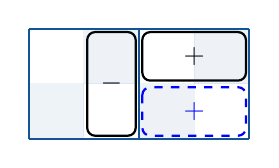
\begin{tikzpicture}[tableau, scale = .7]
        \gridLines{1}{2}
        \verticalDomino{1}{2}{-}
        \horizontalDomino{1}{3}{+}
        \horizontalDominoMaybe{2}{3}{+}
        \fixedSquaresForGrid{1}{2}
      \end{tikzpicture}}}
      \quad\text{or}\quad
      \vcenter{\hbox{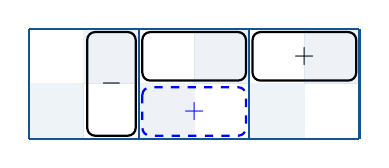
\begin{tikzpicture}[tableau, scale = .7]
        \gridLines{1}{3}
        \verticalDomino{1}{2}{-}
        \horizontalDomino{1}{3}{}
        \horizontalDomino{1}{5}{+}
        \horizontalDominoMaybe{2}{3}{+}
        \fixedSquaresForGrid{1}{3}
      \end{tikzpicture}}}
    \end{equation*}
    \item If the pair domino has the same sign, we need to see if there is a blank domino in the same column.
    Concretely, we call the function \texttt{findSignInRowRight()} on the corresponding row in the dual sign tableau.
    \begin{itemize}
      \item If \texttt{findSignInRowRight()} doesn't find a sign (or if we didn't bother to call the function because there's only one domino in the column), that means that our column is full of $+$ signs.
      We look next at the row below the end of this column.
      \begin{figure}[H]
        \centering
        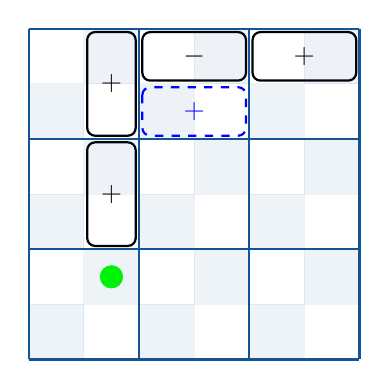
\begin{tikzpicture}[tableau, scale = .7]
          \gridLines{3}{3}
          \verticalDomino{1}{2}{+}
          \horizontalDomino{1}{3}{-}
          \horizontalDomino{1}{5}{+}
          \horizontalDominoMaybe{2}{3}{+}
          \verticalDomino{3}{2}{+}
          \greenCircle{5}{2}
          \fixedSquaresForGrid{3}{3}
        \end{tikzpicture}
      \end{figure}
      \item If \texttt{findSignInRowRight()} finds a sign, we'll interchange the signs.
      We'll do the preparation and move the signs in this function.
      (Note, some of these cases can be complicated, possibly related to complicated cases of adding the first number.
      See the first example in examples.txt.
      This needs further examination.)
      Also, I think after this interchange, we're done here, but I'm not sure.
      In the code, the function proceeds.
      So, this also needs further examination.
      Here is a basic example of the interchange.
      \begin{figure}[H]
        \centering
        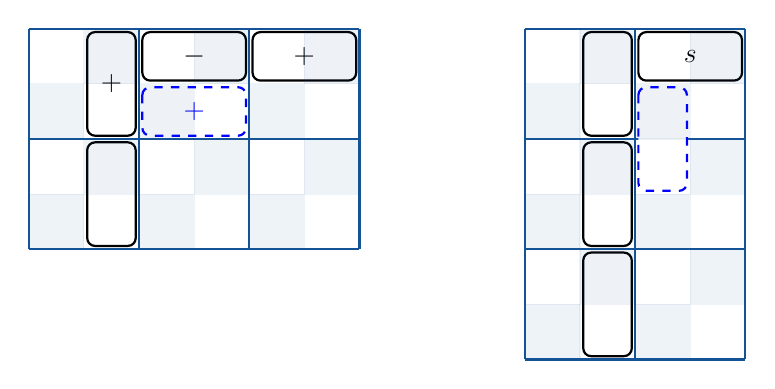
\begin{tikzpicture}[tableau, scale = .7]
          \gridLines{2}{3}
          \verticalDomino{1}{2}{+}
          \horizontalDomino{1}{3}{-}
          \horizontalDomino{1}{5}{+}
          \horizontalDominoMaybe{2}{3}{+}
          \verticalDomino{3}{2}{}
          \fixedSquaresForGrid{2}{3}

          \gridLinesShift{3}{2}{9}
          \verticalDominoShift{1}{2}{ }{9}
          \horizontalDominoShift{1}{3}{s}{9}
          \verticalDominoShift{3}{2}{ }{9}
          \verticalDominoShift{5}{2}{ }{9}
          \verticalDominoMaybeShift{2}{3}{ }{9}
          \fixedSquaresForGridShift{3}{2}{9}
        \end{tikzpicture}
      \end{figure}
      goes to
      \begin{figure}[H]
        \centering
        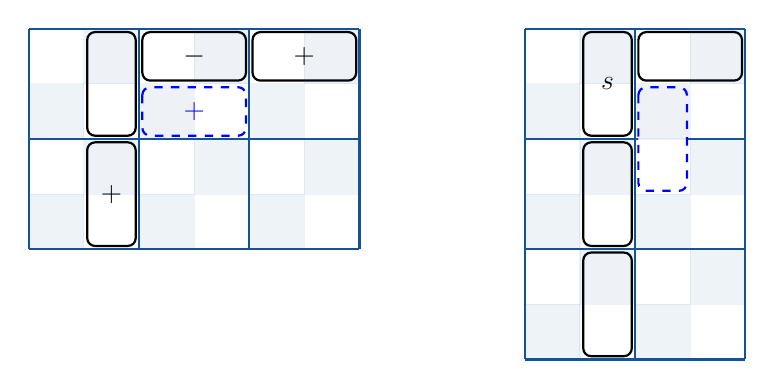
\begin{tikzpicture}[tableau, scale = .7]
          \gridLines{2}{3}
          \verticalDomino{1}{2}{}
          \horizontalDomino{1}{3}{-}
          \horizontalDomino{1}{5}{+}
          \horizontalDominoMaybe{2}{3}{+}
          \verticalDomino{3}{2}{+}
          \fixedSquaresForGrid{2}{3}

          \gridLinesShift{3}{2}{9}
          \verticalDominoShift{1}{2}{s}{9}
          \horizontalDominoShift{1}{3}{}{9}
          \verticalDominoShift{3}{2}{ }{9}
          \verticalDominoShift{5}{2}{ }{9}
          \verticalDominoMaybeShift{2}{3}{ }{9}
          \fixedSquaresForGridShift{3}{2}{9}
        \end{tikzpicture}
      \end{figure}

      At this point in the function (whether or not we made an interchange) we have a blank, vertical domino as the pair domino.
      However, that isn't good enough.
      I think, at this point, there's a sign in the row above.
      We use \texttt{findSignInRowRight()} to find the sign.
      If it's a $-$ sign, then we're good to go.
      We can use it to cancel the $+$ sign which we are adding.
      So, we return this row as the row to add the $+$ sign.
      \begin{figure}[H]
        \centering
        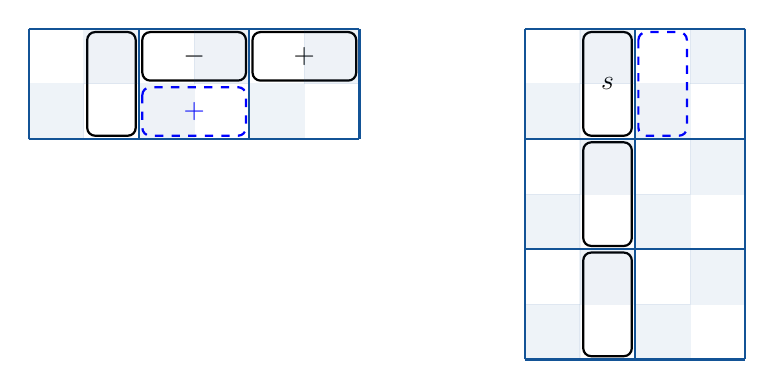
\begin{tikzpicture}[tableau, scale = .7]
          \gridLines{1}{3}
          \verticalDomino{1}{2}{}
          \horizontalDomino{1}{3}{-}
          \horizontalDomino{1}{5}{+}
          \horizontalDominoMaybe{2}{3}{+}
          \fixedSquaresForGrid{1}{3}

          \gridLinesShift{3}{2}{9}
          \verticalDominoShift{1}{2}{s}{9}
          \verticalDominoShift{3}{2}{ }{9}
          \verticalDominoShift{5}{2}{ }{9}
          \verticalDominoMaybeShift{1}{3}{ }{9}
          \fixedSquaresForGridShift{3}{2}{9}
        \end{tikzpicture}
      \end{figure}
      or
      \begin{figure}[H]
        \centering
        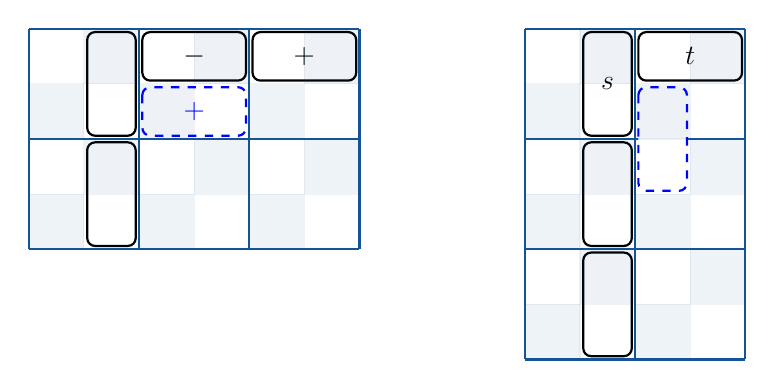
\begin{tikzpicture}[tableau, scale = .7]
          \gridLines{2}{3}
          \verticalDomino{1}{2}{}
          \horizontalDomino{1}{3}{-}
          \horizontalDomino{1}{5}{+}
          \horizontalDominoMaybe{2}{3}{+}
          \verticalDomino{3}{2}{}
          \fixedSquaresForGrid{2}{3}

          \gridLinesShift{3}{2}{9}
          \verticalDominoShift{1}{2}{s}{9}
          \horizontalDominoShift{1}{3}{t}{9}
          \verticalDominoShift{3}{2}{ }{9}
          \verticalDominoShift{5}{2}{ }{9}
          \verticalDominoMaybeShift{2}{3}{ }{9}
          \fixedSquaresForGridShift{3}{2}{9}
        \end{tikzpicture}
      \end{figure}

      If on the other hand, it's a $+$ sign, then we are going to need another blank domino in the column to the left.
      We'll need to put the $+$ sign there.
      If there are no more dominoes in the column, we can't add here.
      We return the next row to add at.
      \begin{figure}[H]
        \centering
        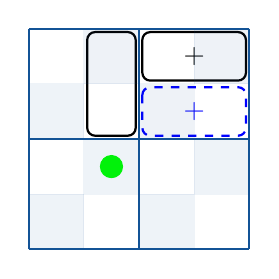
\begin{tikzpicture}[tableau, scale = .7]
          \gridLines{2}{2}
          \verticalDomino{1}{2}{}
          \horizontalDomino{1}{3}{+}
          \horizontalDominoMaybe{2}{3}{+}
          \greenCircle{3}{2}
          \fixedSquaresForGrid{2}{2}
        \end{tikzpicture}
      \end{figure}

      Otherwise, to find out which case we are in, and to prepare for placing the sign, we call \texttt{findRowToAddSignX()} at the next row down (and the same column).

      Here is a simple positive example.
      \begin{figure}[H]
        \centering
        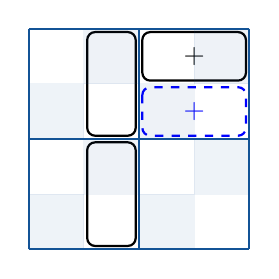
\begin{tikzpicture}[tableau, scale = .7]
          \gridLines{2}{2}
          \verticalDomino{1}{2}{}
          \horizontalDomino{1}{3}{+}
          \horizontalDominoMaybe{2}{3}{+}
          \verticalDomino{3}{2}{}
          \fixedSquaresForGrid{2}{2}
        \end{tikzpicture}
      \end{figure}

      The function \texttt{findRowToAddSignX()} doesn't do all the switching which we need for this situation.
      There may be a domino with a $-$ sign at the bottom of the column, in a horizontal domino.
      Since the minus sign is not up, we know that we can switch it left, and we do that here.
      Then, later, we can put a $+$ sign in its place.

      Here is an example.
      \begin{figure}[H]
        \centering
        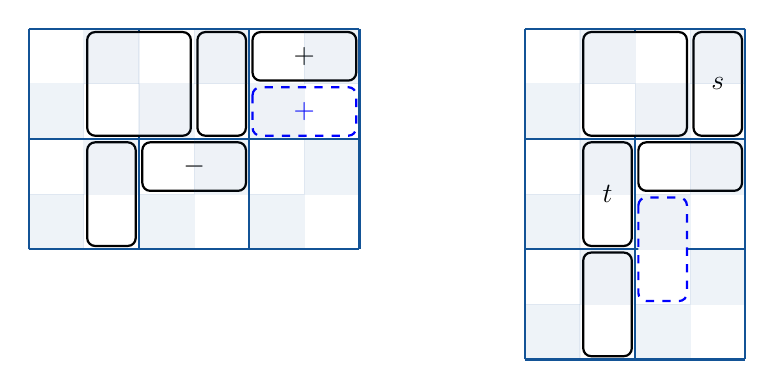
\begin{tikzpicture}[tableau, scale = .7]
          \gridLines{2}{3}
          \emptyBox{1}{2}
          \verticalDomino{1}{4}{}
          \horizontalDomino{1}{5}{+}
          \horizontalDominoMaybe{2}{5}{+}
          \horizontalDomino{3}{3}{-}
          \verticalDomino{3}{2}{}
          \fixedSquaresForGrid{2}{3}

          \gridLinesShift{3}{2}{9}
          \emptyBoxShift{1}{2}{9}
          \verticalDominoShift{1}{4}{s}{9}
          \verticalDominoShift{3}{2}{t}{9}
          \horizontalDominoShift{3}{3}{}{9}
          \verticalDominoShift{5}{2}{ }{9}
          \verticalDominoMaybeShift{4}{3}{ }{9}
          \fixedSquaresForGridShift{3}{2}{9}
        \end{tikzpicture}
      \end{figure}
      goes to
      \begin{figure}[H]
        \centering
        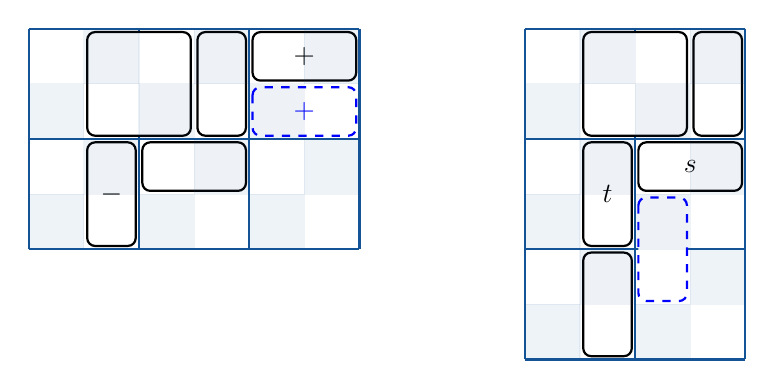
\begin{tikzpicture}[tableau, scale = .7]
          \gridLines{2}{3}
          \emptyBox{1}{2}
          \verticalDomino{1}{4}{}
          \horizontalDomino{1}{5}{+}
          \horizontalDominoMaybe{2}{5}{+}
          \horizontalDomino{3}{3}{}
          \verticalDomino{3}{2}{-}
          \fixedSquaresForGrid{2}{3}

          \gridLinesShift{3}{2}{9}
          \emptyBoxShift{1}{2}{9}
          \verticalDominoShift{1}{4}{}{9}
          \verticalDominoShift{3}{2}{t}{9}
          \horizontalDominoShift{3}{3}{s}{9}
          \verticalDominoShift{5}{2}{}{9}
          \verticalDominoMaybeShift{4}{3}{ }{9}
          \fixedSquaresForGridShift{3}{2}{9}
        \end{tikzpicture}
      \end{figure}
    \end{itemize}
  \end{itemize}

  Now we can do the cases for grid position $Z$.
  Our top-level cases will be whether the pair domino is horizontal or not.
  \begin{itemize}
    \item Here the pair domino is horizontal.
    The pair domino is then a cycle top.
    The adjacent domino (to the left) is also horizontal, as part (in fact an end) of the cycle.
    Now we break into cases based on the sign in the pair domino.
    \begin{itemize}
      \item Here the pair domino has a $+$ sign.
      Then the adjacent domino has effective sign $+$ as well, and we can't add at this level.
      However, the next row down is shorter than this one, so we move there and try to add there.
      \item Here the pair domino has a $-$ sign.
      Then the adjacent domino has effective sign $-$.
      Its actual sign is either $-$ or blank.
      \begin{itemize}
        \item Here the adjacent domino has a $-$ sign.
        We can just add the new domino here, with its $+$ sign, as a horizontal domino.
        \begin{figure}[H]
          \centering
          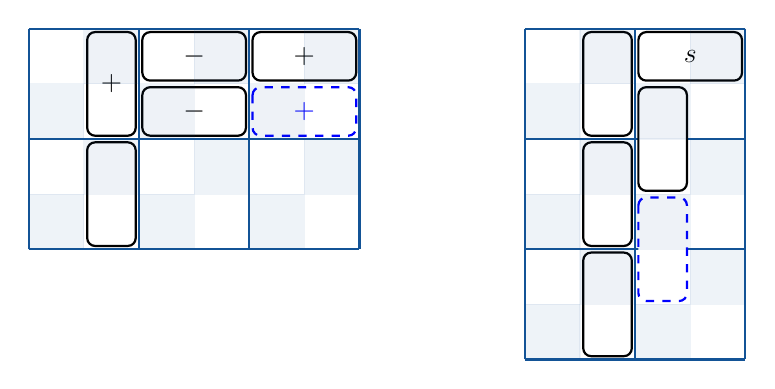
\begin{tikzpicture}[tableau, scale = .7]
            \gridLines{2}{3}
            \verticalDomino{1}{2}{+}
            \horizontalDomino{1}{3}{-}
            \horizontalDomino{2}{3}{-}
            \horizontalDomino{1}{5}{+}
            \verticalDomino{3}{2}{ }
            \horizontalDominoMaybe{2}{5}{+}
            \fixedSquaresForGrid{2}{3}

            \gridLinesShift{3}{2}{9}
            \verticalDominoShift{1}{2}{ }{9}
            \horizontalDominoShift{1}{3}{s}{9}
            \verticalDominoShift{3}{2}{ }{9}
            \verticalDominoShift{2}{3}{ }{9}
            \verticalDominoShift{5}{2}{ }{9}
            \verticalDominoMaybeShift{4}{3}{ }{9}
            \fixedSquaresForGridShift{3}{2}{9}
          \end{tikzpicture}
        \end{figure}

        \begin{figure}[H]
          \centering
          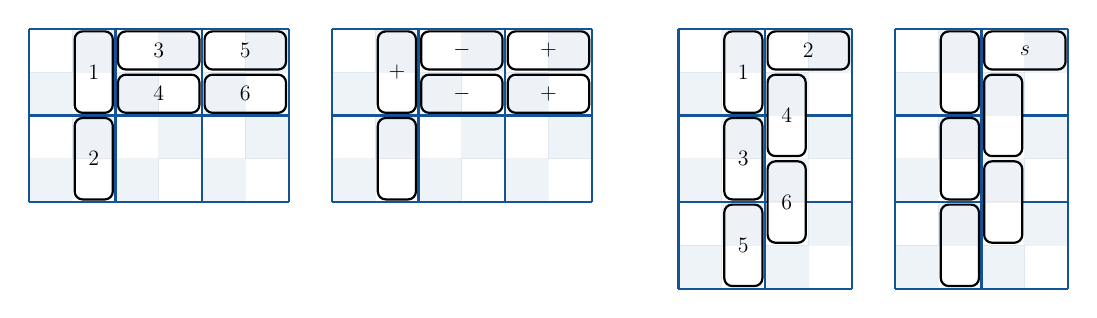
\begin{tikzpicture}[tableau, scale=.55]\gridLines{2}{3}\verticalDomino{1}{2}{1}\verticalDomino{3}{2}{2}\horizontalDomino{1}{3}{3}\horizontalDomino{2}{3}{4}\horizontalDomino{1}{5}{5}\horizontalDomino{2}{5}{6}\fixedSquaresForGrid{2}{3}\gridLinesShift{2}{3}{7}\verticalDominoShift{1}{2}{+}{7}\verticalDominoShift{3}{2}{}{7}\horizontalDominoShift{1}{3}{-}{7}\horizontalDominoShift{2}{3}{-}{7}\horizontalDominoShift{1}{5}{+}{7}\horizontalDominoShift{2}{5}{+}{7}\fixedSquaresForGridShift{2}{3}{7}\gridLinesShift{3}{2}{15}\verticalDominoShift{1}{2}{1}{15}\horizontalDominoShift{1}{3}{2}{15}\verticalDominoShift{3}{2}{3}{15}\verticalDominoShift{2}{3}{4}{15}\verticalDominoShift{5}{2}{5}{15}\verticalDominoShift{4}{3}{6}{15}\fixedSquaresForGridShift{3}{2}{15}\gridLinesShift{3}{2}{20}\verticalDominoShift{1}{2}{}{20}\horizontalDominoShift{1}{3}{s}{20}\verticalDominoShift{3}{2}{}{20}\verticalDominoShift{2}{3}{}{20}\verticalDominoShift{5}{2}{}{20}\verticalDominoShift{4}{3}{}{20}\fixedSquaresForGridShiftAlt{3}{2}{20}\end{tikzpicture}
        \end{figure}
        \item Here the adjacent domino is blank.
        \begin{figure}[H]
          \centering
          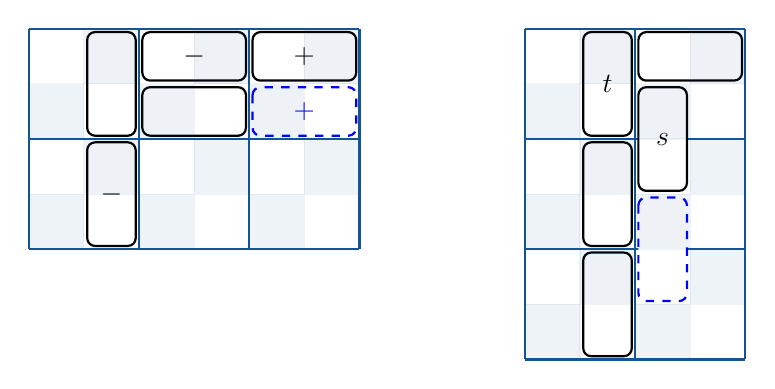
\begin{tikzpicture}[tableau, scale = .7]
            \gridLines{2}{3}
            \verticalDomino{1}{2}{ }
            \horizontalDomino{1}{3}{-}
            \horizontalDomino{2}{3}{ }
            \horizontalDomino{1}{5}{+}
            \verticalDomino{3}{2}{-}
            \horizontalDominoMaybe{2}{5}{+}
            \fixedSquaresForGrid{2}{3}

            \gridLinesShift{3}{2}{9}
            \verticalDominoShift{1}{2}{t}{9}
            \horizontalDominoShift{1}{3}{ }{9}
            \verticalDominoShift{3}{2}{ }{9}
            \verticalDominoShift{2}{3}{s}{9}
            \verticalDominoShift{5}{2}{ }{9}
            \verticalDominoMaybeShift{4}{3}{ }{9}
            \fixedSquaresForGridShift{3}{2}{9}
          \end{tikzpicture}
        \end{figure}
        We can still add the domino here, as a horizontal domino.
        But, this time its sign is on the dual side.
        We also need to blank out the pair domino on this side, and give the corresponding domino on the dual side the appropriate sign.
        \begin{figure}[H]
          \centering
          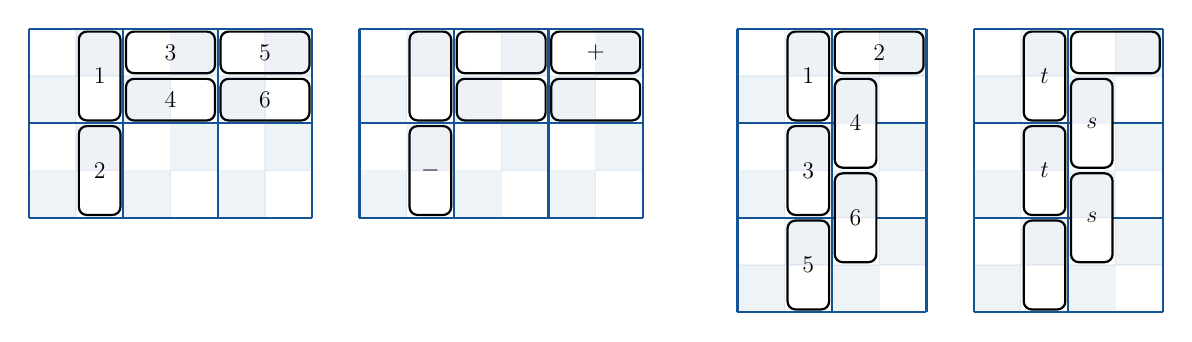
\begin{tikzpicture}[tableau, scale=.6]\gridLines{2}{3}\verticalDomino{1}{2}{1}\verticalDomino{3}{2}{2}\horizontalDomino{1}{3}{3}\horizontalDomino{2}{3}{4}\horizontalDomino{1}{5}{5}\horizontalDomino{2}{5}{6}\fixedSquaresForGrid{2}{3}\gridLinesShift{2}{3}{7}\verticalDominoShift{1}{2}{}{7}\verticalDominoShift{3}{2}{-}{7}\horizontalDominoShift{1}{3}{}{7}\horizontalDominoShift{2}{3}{}{7}\horizontalDominoShift{1}{5}{+}{7}\horizontalDominoShift{2}{5}{}{7}\fixedSquaresForGridShift{2}{3}{7}\gridLinesShift{3}{2}{15}\verticalDominoShift{1}{2}{1}{15}\horizontalDominoShift{1}{3}{2}{15}\verticalDominoShift{3}{2}{3}{15}\verticalDominoShift{2}{3}{4}{15}\verticalDominoShift{5}{2}{5}{15}\verticalDominoShift{4}{3}{6}{15}\fixedSquaresForGridShift{3}{2}{15}\gridLinesShift{3}{2}{20}\verticalDominoShift{1}{2}{t}{20}\horizontalDominoShift{1}{3}{}{20}\verticalDominoShift{3}{2}{t}{20}\verticalDominoShift{2}{3}{s}{20}\verticalDominoShift{5}{2}{}{20}\verticalDominoShift{4}{3}{s}{20}\fixedSquaresForGridShiftAlt{3}{2}{20}\end{tikzpicture}
        \end{figure}
      \end{itemize}
      \item Here the pair domino is blank.
      However, there must be some sign in the row above, for us to have come down this far.
      We need to know the effective sign, that is, the leftmost sign.
      We call \texttt{findSignInRowRight()} to get that information.
      \begin{itemize}
        \item Here the effective sign is $+$.
        Then we can't add the domino to this row.
        Instead, we go to the next row down.
        \item Here the effective sign is $-$.
        \begin{figure}[H]
          \centering
          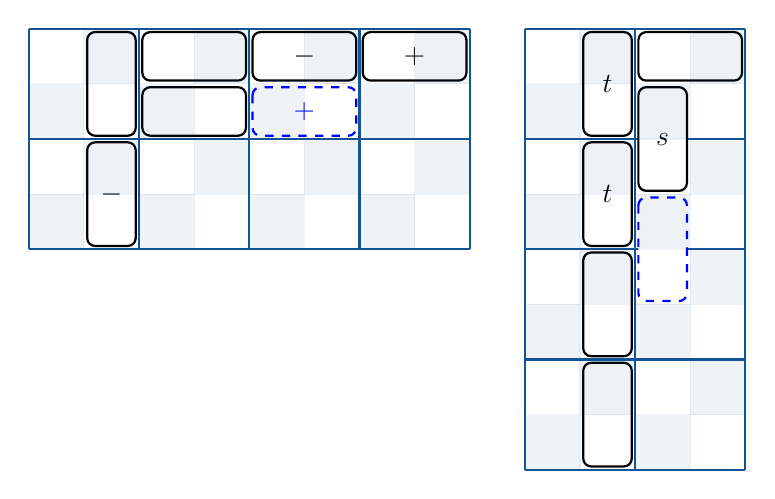
\begin{tikzpicture}[tableau, scale = .7]
            \gridLines{2}{4}
            \verticalDomino{1}{2}{ }
            \horizontalDomino{1}{3}{ }
            \horizontalDomino{2}{3}{ }
            \horizontalDomino{1}{5}{-}
            \horizontalDomino{1}{7}{+}
            \verticalDomino{3}{2}{-}
            \horizontalDominoMaybe{2}{5}{+}
            \fixedSquaresForGrid{2}{4}

            \gridLinesShift{4}{2}{9}
            \verticalDominoShift{1}{2}{t}{9}
            \horizontalDominoShift{1}{3}{ }{9}
            \verticalDominoShift{3}{2}{t}{9}
            \verticalDominoShift{2}{3}{s}{9}
            \verticalDominoShift{5}{2}{ }{9}
            \verticalDominoShift{7}{2}{ }{9}
            \verticalDominoMaybeShift{4}{3}{ }{9}
            \fixedSquaresForGridShift{4}{2}{9}
          \end{tikzpicture}
        \end{figure}
        So, we can add the domino at this level.
        However, it will come in as a blank domino, and we also need to cancel the sign of the domino holding the $-$, and to put appropriate signs into the corresponding dominoes in the other sign tableau.
        \begin{figure}[H]
          \centering
          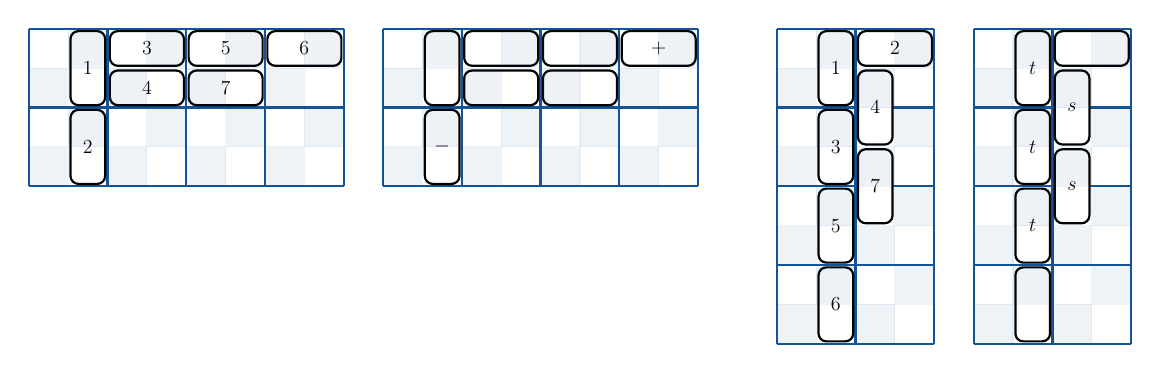
\begin{tikzpicture}[tableau, scale=.5]\gridLines{2}{4}\verticalDomino{1}{2}{1}\verticalDomino{3}{2}{2}\horizontalDomino{1}{3}{3}\horizontalDomino{2}{3}{4}\horizontalDomino{1}{5}{5}\horizontalDomino{1}{7}{6}\horizontalDomino{2}{5}{7}\fixedSquaresForGrid{2}{4}\gridLinesShift{2}{4}{9}\verticalDominoShift{1}{2}{}{9}\verticalDominoShift{3}{2}{-}{9}\horizontalDominoShift{1}{3}{}{9}\horizontalDominoShift{2}{3}{}{9}\horizontalDominoShift{1}{5}{}{9}\horizontalDominoShift{1}{7}{+}{9}\horizontalDominoShift{2}{5}{}{9}\fixedSquaresForGridShift{2}{4}{9}\gridLinesShift{4}{2}{19}\verticalDominoShift{1}{2}{1}{19}\horizontalDominoShift{1}{3}{2}{19}\verticalDominoShift{3}{2}{3}{19}\verticalDominoShift{2}{3}{4}{19}\verticalDominoShift{5}{2}{5}{19}\verticalDominoShift{7}{2}{6}{19}\verticalDominoShift{4}{3}{7}{19}\fixedSquaresForGridShift{4}{2}{19}\gridLinesShift{4}{2}{24}\verticalDominoShift{1}{2}{t}{24}\horizontalDominoShift{1}{3}{}{24}\verticalDominoShift{3}{2}{t}{24}\verticalDominoShift{2}{3}{s}{24}\verticalDominoShift{5}{2}{t}{24}\verticalDominoShift{7}{2}{}{24}\verticalDominoShift{4}{3}{s}{24}\fixedSquaresForGridShiftAlt{4}{2}{24}\end{tikzpicture}
        \end{figure}

        Since we are putting a sign into the opposite domino of the domino with a $-$ sign, there may be some issues if that domino is horizontal.
        (Note, it seems like this only happens when that horizontal domino just came down as part of inserting a pair.)
        We can still place the sign for sure, but we need to handle the issues.
        The function \texttt{prepareForSign()} will do that.

        There are two possible issues.
        On the one hand, the domino may be at the top of a cycle, in which case \texttt{prepareForSign()} will call \texttt{putSignInCycleTop()}.
        (Right now, this looks toatlly routine, so I won't do an example.)
        On the other hand, there may be a domino of the same sign in the row.
        Now, the sign which we are putting in the domino is already in its column.
        So, there can't a horizontal domino of that sign in the row, since else it would have moved to the position occupied by the domino which we are putting the sign into.
        So, the only possibility is that there is a vertical domino with that sign in the row.
        So, \texttt{prepareForSign()} will call \texttt{makeSpaceFor()} to move that domino down, if it is there.
        \begin{figure}[H]
          \centering
          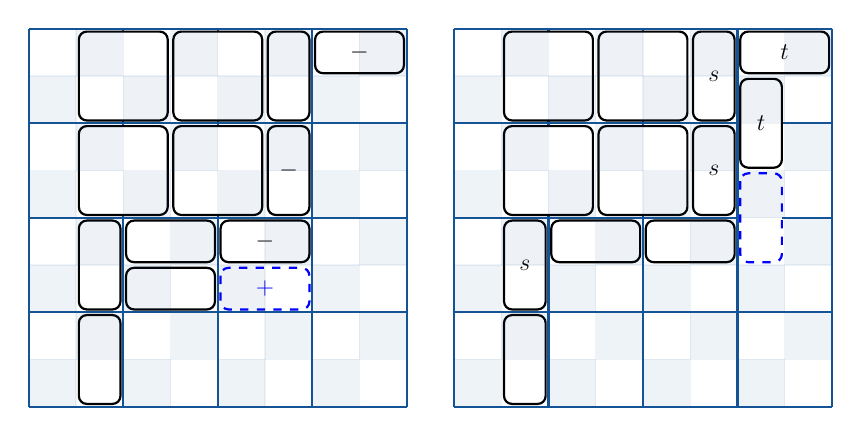
\begin{tikzpicture}[tableau, scale = .6]
            \gridLines{4}{4}
            \emptyBox{1}{2}
            \emptyBox{1}{4}
            \emptyBox{3}{2}
            \emptyBox{3}{4}
            \verticalDomino{1}{6}{ }
            \horizontalDomino{1}{7}{-}
            \verticalDomino{3}{6}{-}
            \verticalDomino{5}{2}{ }
            \verticalDomino{7}{2}{ }
            \horizontalDomino{5}{3}{ }
            \horizontalDomino{6}{3}{ }
            \horizontalDomino{5}{5}{-}
            \horizontalDominoMaybe{6}{5}{+}
            \fixedSquaresForGrid{4}{4}

            \gridLinesShift{4}{4}{9}
            \emptyBoxShift{1}{2}{9}
            \emptyBoxShift{1}{4}{9}
            \emptyBoxShift{3}{2}{9}
            \emptyBoxShift{3}{4}{9}
            \verticalDominoShift{1}{6}{s}{9}
            \verticalDominoShift{3}{6}{s}{9}
            \verticalDominoShift{2}{7}{t}{9}
            \verticalDominoShift{5}{2}{s}{9}
            \verticalDominoShift{7}{2}{}{9}
            \horizontalDominoShift{1}{7}{t}{9}
            \horizontalDominoShift{5}{3}{}{9}
            \horizontalDominoShift{5}{5}{}{9}
            \verticalDominoMaybeShift{4}{7}{ }{9}
            \fixedSquaresForGridShift{4}{4}{9}
          \end{tikzpicture}
        \end{figure}

        \begin{figure}[H]
          \centering
          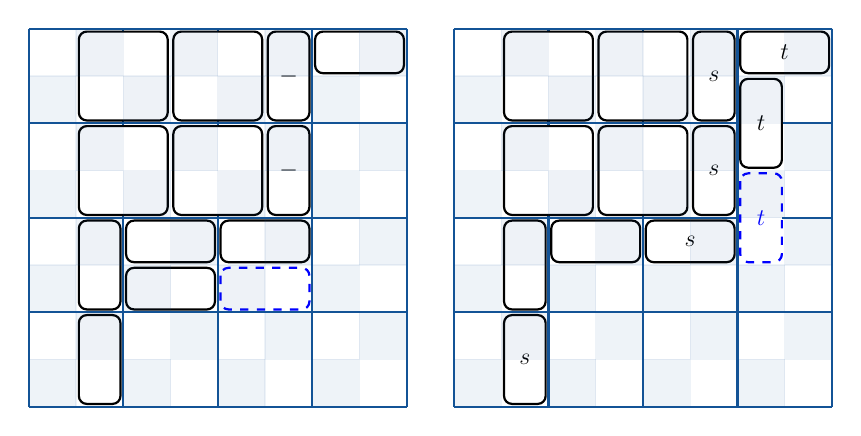
\begin{tikzpicture}[tableau, scale = .6]
            \gridLines{4}{4}
            \emptyBox{1}{2}
            \emptyBox{1}{4}
            \emptyBox{3}{2}
            \emptyBox{3}{4}
            \verticalDomino{1}{6}{-}
            \horizontalDomino{1}{7}{}
            \verticalDomino{3}{6}{-}
            \verticalDomino{5}{2}{ }
            \verticalDomino{7}{2}{ }
            \horizontalDomino{5}{3}{ }
            \horizontalDomino{6}{3}{ }
            \horizontalDomino{5}{5}{}
            \horizontalDominoMaybe{6}{5}{}
            \fixedSquaresForGrid{4}{4}

            \gridLinesShift{4}{4}{9}
            \emptyBoxShift{1}{2}{9}
            \emptyBoxShift{1}{4}{9}
            \emptyBoxShift{3}{2}{9}
            \emptyBoxShift{3}{4}{9}
            \verticalDominoShift{1}{6}{s}{9}
            \verticalDominoShift{3}{6}{s}{9}
            \verticalDominoShift{2}{7}{t}{9}
            \verticalDominoShift{5}{2}{}{9}
            \verticalDominoShift{7}{2}{s}{9}
            \horizontalDominoShift{1}{7}{t}{9}
            \horizontalDominoShift{5}{3}{}{9}
            \horizontalDominoShift{5}{5}{s}{9}
            \verticalDominoMaybeShift{4}{7}{t}{9}
            \fixedSquaresForGridShift{4}{4}{9}
          \end{tikzpicture}
        \end{figure}

        \begin{figure}[H]
          \centering
          % 5- 2_6 7+ 8+ 9s 4_11 10_-12 13- 1_14 15- 16- 3_17
          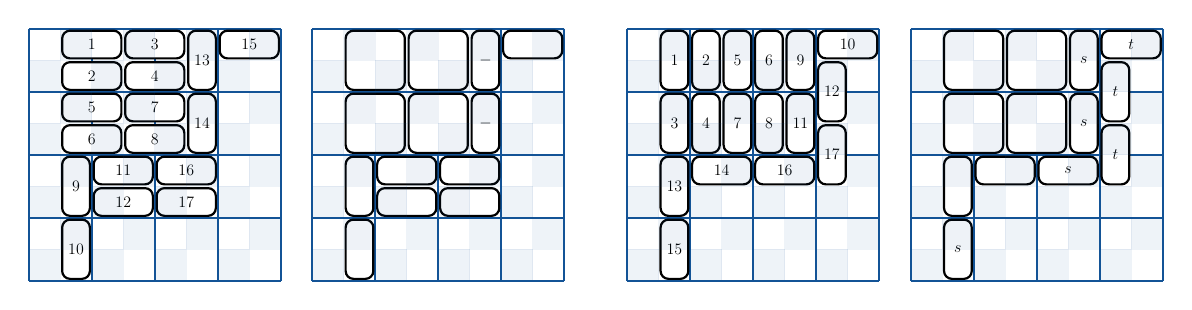
\begin{tikzpicture}[tableau, scale=.4]\gridLines{4}{4}\horizontalDomino{1}{2}{1}\horizontalDomino{2}{2}{2}\horizontalDomino{1}{4}{3}\horizontalDomino{2}{4}{4}\horizontalDomino{3}{2}{5}\horizontalDomino{4}{2}{6}\horizontalDomino{3}{4}{7}\horizontalDomino{4}{4}{8}\verticalDomino{5}{2}{9}\verticalDomino{7}{2}{10}\horizontalDomino{5}{3}{11}\horizontalDomino{6}{3}{12}\verticalDomino{1}{6}{13}\verticalDomino{3}{6}{14}\horizontalDomino{1}{7}{15}\horizontalDomino{5}{5}{16}\horizontalDomino{6}{5}{17}\fixedSquaresForGrid{4}{4}\gridLinesShift{4}{4}{9}\emptyBoxShift{1}{2}{9}\verticalDominoShift{5}{2}{}{9}\emptyBoxShift{1}{4}{9}\verticalDominoShift{7}{2}{}{9}\horizontalDominoShift{5}{3}{}{9}\emptyBoxShift{3}{2}{9}\verticalDominoShift{1}{6}{-}{9}\horizontalDominoShift{6}{3}{}{9}\verticalDominoShift{3}{6}{-}{9}\horizontalDominoShift{1}{7}{}{9}\horizontalDominoShift{5}{5}{}{9}\emptyBoxShift{3}{4}{9}\horizontalDominoShift{6}{5}{}{9}\fixedSquaresForGridShift{4}{4}{9}\gridLinesShift{4}{4}{19}\verticalDominoShift{1}{2}{1}{19}\verticalDominoShift{1}{3}{2}{19}\verticalDominoShift{3}{2}{3}{19}\verticalDominoShift{3}{3}{4}{19}\verticalDominoShift{1}{4}{5}{19}\verticalDominoShift{1}{5}{6}{19}\verticalDominoShift{3}{4}{7}{19}\verticalDominoShift{3}{5}{8}{19}\verticalDominoShift{1}{6}{9}{19}\horizontalDominoShift{1}{7}{10}{19}\verticalDominoShift{3}{6}{11}{19}\verticalDominoShift{2}{7}{12}{19}\verticalDominoShift{5}{2}{13}{19}\horizontalDominoShift{5}{3}{14}{19}\verticalDominoShift{7}{2}{15}{19}\horizontalDominoShift{5}{5}{16}{19}\verticalDominoShift{4}{7}{17}{19}\fixedSquaresForGridShift{4}{4}{19}\gridLinesShift{4}{4}{28}\emptyBoxShift{1}{2}{28}\verticalDominoShift{1}{6}{s}{28}\emptyBoxShift{3}{2}{28}\horizontalDominoShift{1}{7}{t}{28}\verticalDominoShift{3}{6}{s}{28}\emptyBoxShift{1}{4}{28}\verticalDominoShift{5}{2}{}{28}\verticalDominoShift{2}{7}{t}{28}\horizontalDominoShift{5}{3}{}{28}\verticalDominoShift{7}{2}{s}{28}\horizontalDominoShift{5}{5}{s}{28}\emptyBoxShift{3}{4}{28}\verticalDominoShift{4}{7}{t}{28}\fixedSquaresForGridShiftAlt{4}{4}{28}\end{tikzpicture}
        \end{figure}
      \end{itemize}
    \end{itemize}
    \item Here the pair domino is vertical.
    If the pair domino has a plus sign, we might not be able to add at this level.
    OTOH, we might be able to move such a domino down.
    The function \texttt{findRowToAddSignZ()} takes care of the situation.
    Based on its output, we may have to add at a lower level.

    Henceforth, assume we can add at this level.
    The two cases depend on the length of the next row.
    \begin{itemize}
      \item Here the next row has a smaller length than this row.
      So, we are contracting a type I cycle.
      The two cases depend on the sign in the pair domino.
      \begin{itemize}
        \item Here the pair domino has a $-$ sign.
        We just put the domino and then box it up.
        \begin{figure}[H]
          \centering
          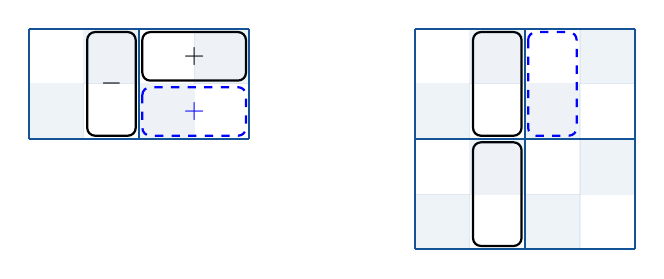
\begin{tikzpicture}[tableau, scale = .7]
            \gridLines{1}{2}
            \verticalDomino{1}{2}{-}
            \horizontalDomino{1}{3}{+}
            \horizontalDominoMaybe{2}{3}{+}
            \fixedSquaresForGrid{1}{2}

            \gridLinesShift{2}{2}{7}
            \verticalDominoShift{1}{2}{ }{7}
            \verticalDominoShift{3}{2}{ }{7}
            \verticalDominoMaybeShift{1}{3}{ }{7}
            \fixedSquaresForGridShift{2}{2}{7}
          \end{tikzpicture}
        \end{figure}

        \begin{figure}[H]
          \centering
          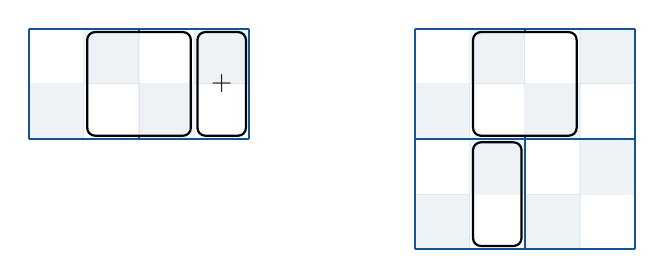
\begin{tikzpicture}[tableau, scale = .7]
            \gridLines{1}{2}
            \emptyBox{1}{2}
            \verticalDomino{1}{4}{+}
            \fixedSquaresForGrid{1}{2}

            \gridLinesShift{2}{2}{7}
            \emptyBoxShift{1}{2}{7}
            \verticalDominoShift{3}{2}{ }{7}
            \fixedSquaresForGridShift{2}{2}{7}
          \end{tikzpicture}
        \end{figure}

        \begin{figure}[H]
          \centering
          % 1- 2+ 3+
          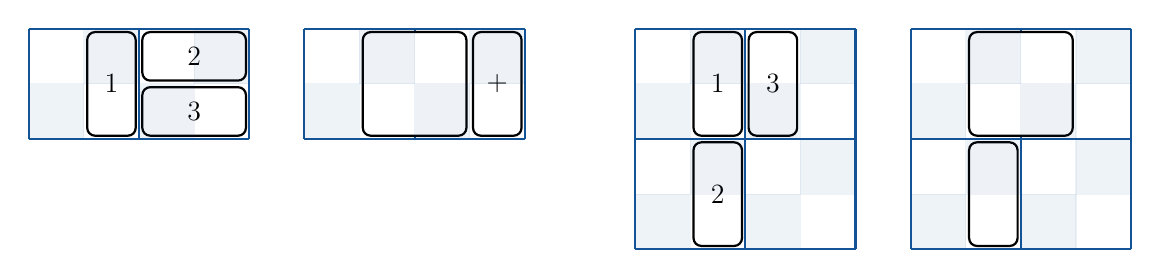
\begin{tikzpicture}[tableau, scale=.7]\gridLines{1}{2}\verticalDomino{1}{2}{1}\horizontalDomino{1}{3}{2}\horizontalDomino{2}{3}{3}\fixedSquaresForGrid{1}{2}\gridLinesShift{1}{2}{5}\verticalDominoShift{1}{4}{+}{5}\emptyBoxShift{1}{2}{5}\fixedSquaresForGridShift{1}{2}{5}\gridLinesShift{2}{2}{11}\verticalDominoShift{1}{2}{1}{11}\verticalDominoShift{3}{2}{2}{11}\verticalDominoShift{1}{3}{3}{11}\fixedSquaresForGridShift{2}{2}{11}\gridLinesShift{2}{2}{16}\verticalDominoShift{3}{2}{}{16}\emptyBoxShift{1}{2}{16}\fixedSquaresForGridShiftAlt{2}{2}{16}\end{tikzpicture}
        \end{figure}
        \item Here the pair domino is blank.
        Then, there is a $-$ sign in the row above, as the leftmost signed domino.
        (TODO, check why this is true.)
        We're going to cancel its sign, which means placing a sign in the corresponding domino on the dual side.
        So, we need \texttt{prepareForSign()}.
        After that, we place dominoes and box them up.
        \begin{figure}[H]
          \centering
          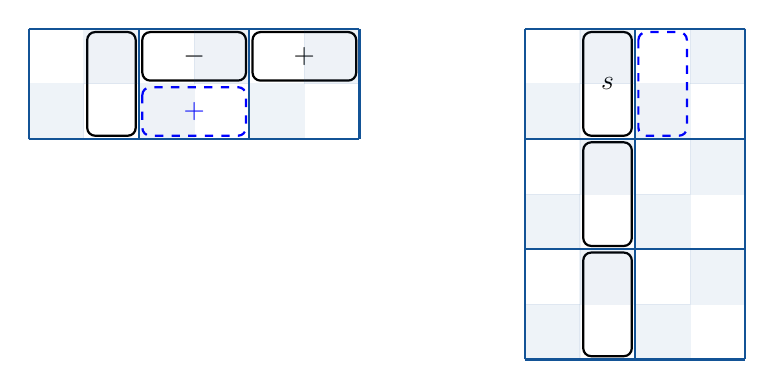
\begin{tikzpicture}[tableau, scale = .7]
            \gridLines{1}{3}
            \verticalDomino{1}{2}{}
            \horizontalDomino{1}{3}{-}
            \horizontalDomino{1}{5}{+}
            \horizontalDominoMaybe{2}{3}{+}
            \fixedSquaresForGrid{1}{3}

            \gridLinesShift{3}{2}{9}
            \verticalDominoShift{1}{2}{s}{9}
            \verticalDominoShift{3}{2}{ }{9}
            \verticalDominoShift{5}{2}{ }{9}
            \verticalDominoMaybeShift{1}{3}{ }{9}
            \fixedSquaresForGridShift{3}{2}{9}
          \end{tikzpicture}
        \end{figure}
        goes to
        \begin{figure}[H]
          \centering
          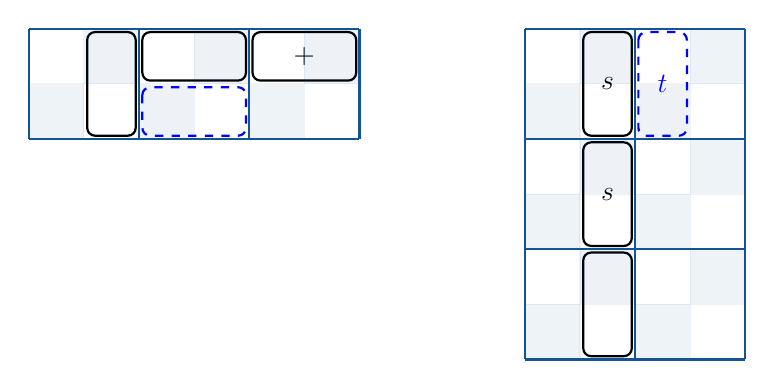
\begin{tikzpicture}[tableau, scale = .7]
            \gridLines{1}{3}
            \verticalDomino{1}{2}{}
            \horizontalDomino{1}{3}{}
            \horizontalDomino{1}{5}{+}
            \horizontalDominoMaybe{2}{3}{}
            \fixedSquaresForGrid{1}{3}

            \gridLinesShift{3}{2}{9}
            \verticalDominoShift{1}{2}{s}{9}
            \verticalDominoShift{3}{2}{s}{9}
            \verticalDominoShift{5}{2}{ }{9}
            \verticalDominoMaybeShift{1}{3}{t}{9}
            \fixedSquaresForGridShift{3}{2}{9}
          \end{tikzpicture}
        \end{figure}
        goes to
        \begin{figure}[H]
          \centering
          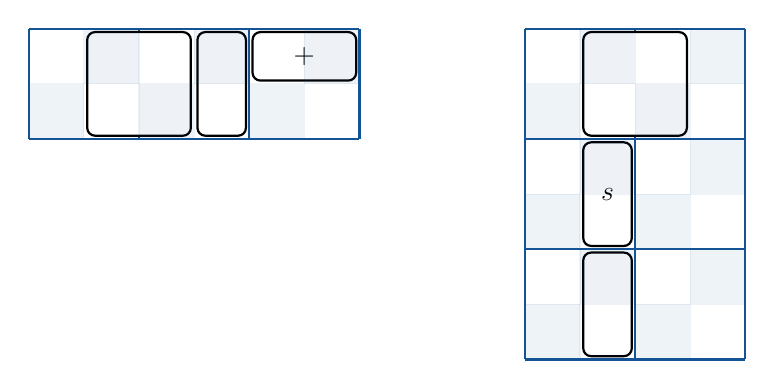
\begin{tikzpicture}[tableau, scale = .7]
            \gridLines{1}{3}
            \emptyBox{1}{2}
            \verticalDomino{1}{4}{}
            \horizontalDomino{1}{5}{+}
            \fixedSquaresForGrid{1}{3}

            \gridLinesShift{3}{2}{9}
            \emptyBoxShift{1}{2}{9}
            \verticalDominoShift{3}{2}{s}{9}
            \verticalDominoShift{5}{2}{ }{9}
            \fixedSquaresForGridShift{3}{2}{9}
          \end{tikzpicture}
        \end{figure}
        \begin{figure}[H]
          % 1s 2- 3+ 4+
          \centering
          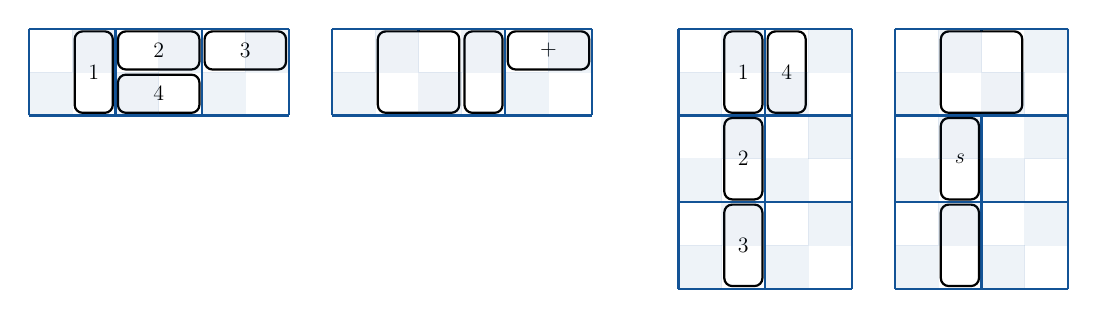
\begin{tikzpicture}[tableau, scale=.55]\gridLines{1}{3}\verticalDomino{1}{2}{1}\horizontalDomino{1}{3}{2}\horizontalDomino{1}{5}{3}\horizontalDomino{2}{3}{4}\fixedSquaresForGrid{1}{3}\gridLinesShift{1}{3}{7}\verticalDominoShift{1}{4}{}{7}\horizontalDominoShift{1}{5}{+}{7}\emptyBoxShift{1}{2}{7}\fixedSquaresForGridShift{1}{3}{7}\gridLinesShift{3}{2}{15}\verticalDominoShift{1}{2}{1}{15}\verticalDominoShift{3}{2}{2}{15}\verticalDominoShift{5}{2}{3}{15}\verticalDominoShift{1}{3}{4}{15}\fixedSquaresForGridShift{3}{2}{15}\gridLinesShift{3}{2}{20}\verticalDominoShift{3}{2}{s}{20}\verticalDominoShift{5}{2}{}{20}\emptyBoxShift{1}{2}{20}\fixedSquaresForGridShiftAlt{3}{2}{20}\end{tikzpicture}
        \end{figure}
      \end{itemize}
      \item  Here the next row has the same length as this row.
      So, we are making a new type II cycle.
      The two cases depend on the sign in the pair domino.
      \begin{itemize}
        \item Here the pair domino has a $-$ sign.
        So, basically, we can put the domino here, with a $+$ sign, since that matches the pair domino.
        However, the configuration may not then be an allowed one for paired cycles, so we may have to adjust for that.
        This depends on what is in the domino just above, and in the domino just below the pair domino.
        Here are the cases.
        \begin{itemize}
          \item If the domino just above has a $+$ sign, we can just put the new domino here, with a $+$ sign.
          \begin{figure}[H]
            \centering
            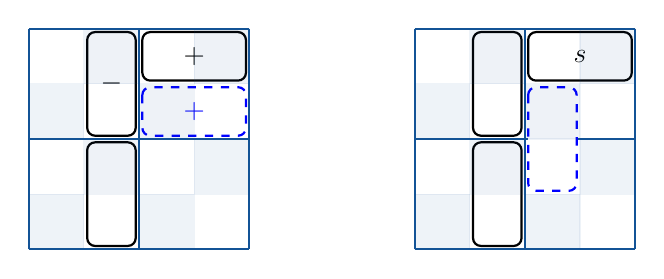
\begin{tikzpicture}[tableau, scale = .7]
              \gridLines{2}{2}
              \verticalDomino{1}{2}{-}
              \horizontalDomino{1}{3}{+}
              \horizontalDominoMaybe{2}{3}{+}
              \verticalDomino{3}{2}{}
              \fixedSquaresForGrid{2}{2}

              \gridLinesShift{2}{2}{7}
              \verticalDominoShift{1}{2}{}{7}
              \horizontalDominoShift{1}{3}{s}{7}
              \verticalDominoShift{3}{2}{ }{7}
              \verticalDominoMaybeShift{2}{3}{ }{7}
              \fixedSquaresForGridShift{2}{2}{7}
            \end{tikzpicture}
          \end{figure}
          \begin{figure}[H]
            % 1- 2s 3+ 4+
            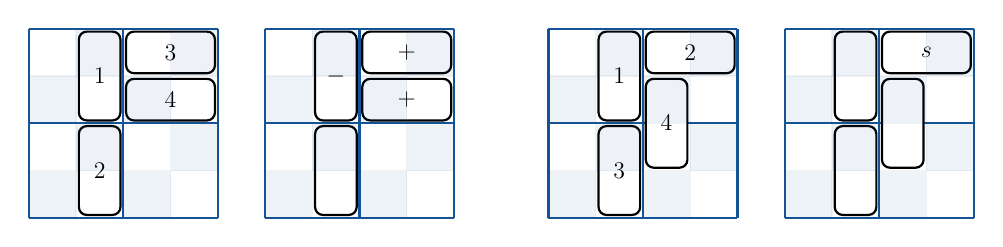
\begin{tikzpicture}[tableau, scale=.6]\gridLines{2}{2}\verticalDomino{1}{2}{1}\verticalDomino{3}{2}{2}\horizontalDomino{1}{3}{3}\horizontalDomino{2}{3}{4}\fixedSquaresForGrid{2}{2}\gridLinesShift{2}{2}{5}\verticalDominoShift{1}{2}{-}{5}\verticalDominoShift{3}{2}{}{5}\horizontalDominoShift{1}{3}{+}{5}\horizontalDominoShift{2}{3}{+}{5}\fixedSquaresForGridShift{2}{2}{5}\gridLinesShift{2}{2}{11}\verticalDominoShift{1}{2}{1}{11}\horizontalDominoShift{1}{3}{2}{11}\verticalDominoShift{3}{2}{3}{11}\verticalDominoShift{2}{3}{4}{11}\fixedSquaresForGridShift{2}{2}{11}\gridLinesShift{2}{2}{16}\verticalDominoShift{1}{2}{}{16}\horizontalDominoShift{1}{3}{s}{16}\verticalDominoShift{3}{2}{}{16}\verticalDominoShift{2}{3}{}{16}\fixedSquaresForGridShiftAlt{2}{2}{16}\end{tikzpicture}
            \centering
          \end{figure}
          \item If the domino just above is blank, we need to check further.
          If the domino just below has a $-$ sign, we can just blank the new domino and the pair domino, and put the appropriate signs in the other side.
          \begin{figure}[H]
            \centering
            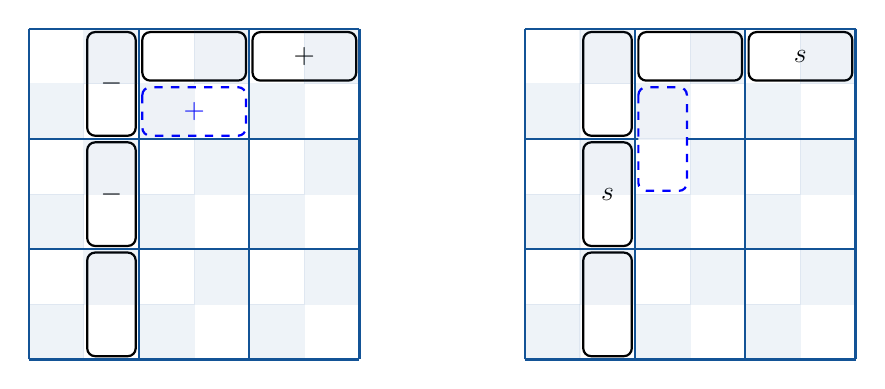
\begin{tikzpicture}[tableau, scale = .7]
              \gridLines{3}{3}
              \verticalDomino{1}{2}{-}
              \horizontalDomino{1}{3}{}
              \horizontalDomino{1}{5}{+}
              \horizontalDominoMaybe{2}{3}{+}
              \verticalDomino{3}{2}{-}
              \verticalDomino{5}{2}{}
              \fixedSquaresForGrid{3}{3}

              \gridLinesShift{3}{3}{9}
              \verticalDominoShift{1}{2}{}{9}
              \horizontalDominoShift{1}{3}{}{9}
              \horizontalDominoShift{1}{5}{s}{9}
              \verticalDominoShift{3}{2}{s}{9}
              \verticalDominoShift{5}{2}{}{9}
              \verticalDominoMaybeShift{2}{3}{ }{9}
              \fixedSquaresForGridShift{3}{3}{9}
            \end{tikzpicture}
          \end{figure}
          goes to
          \begin{figure}[H]
            \centering
            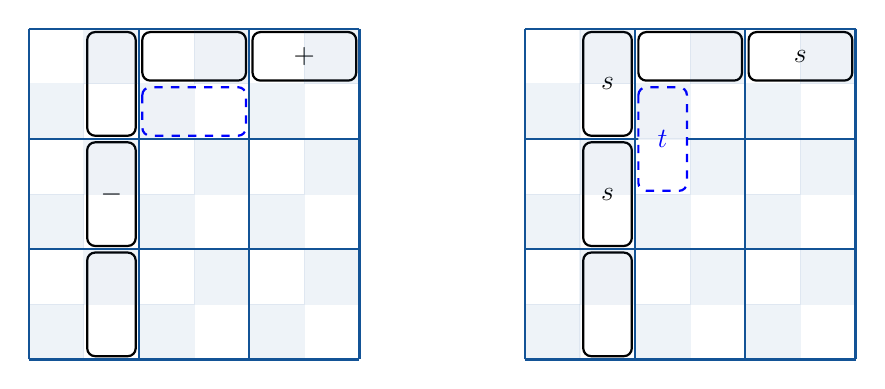
\begin{tikzpicture}[tableau, scale = .7]
              \gridLines{3}{3}
              \verticalDomino{1}{2}{}
              \horizontalDomino{1}{3}{}
              \horizontalDomino{1}{5}{+}
              \horizontalDominoMaybe{2}{3}{}
              \verticalDomino{3}{2}{-}
              \verticalDomino{5}{2}{}
              \fixedSquaresForGrid{3}{3}

              \gridLinesShift{3}{3}{9}
              \verticalDominoShift{1}{2}{s}{9}
              \horizontalDominoShift{1}{3}{}{9}
              \horizontalDominoShift{1}{5}{s}{9}
              \verticalDominoShift{3}{2}{s}{9}
              \verticalDominoShift{5}{2}{}{9}
              \verticalDominoMaybeShift{2}{3}{t}{9}
              \fixedSquaresForGridShift{3}{3}{9}
            \end{tikzpicture}
          \end{figure}
          \begin{figure}[H]
            % 1s 2- 3- 4s 5+ 6+
            \centering
            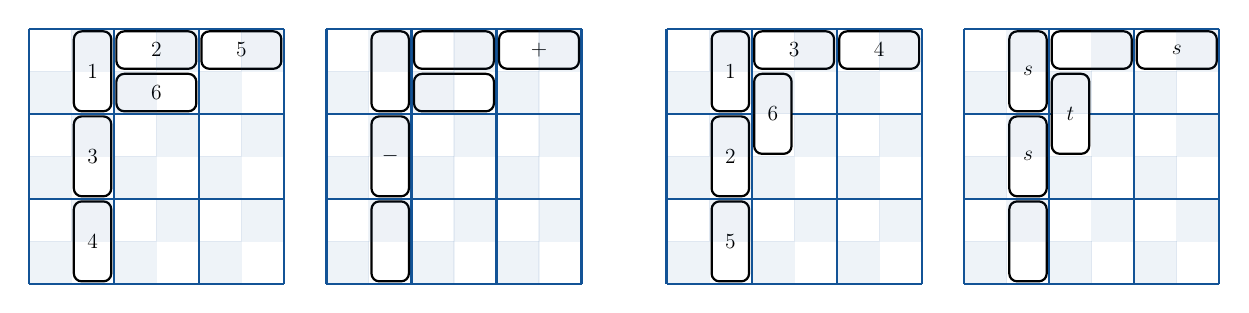
\begin{tikzpicture}[tableau, scale=.54]\gridLines{3}{3}\verticalDomino{1}{2}{1}\horizontalDomino{1}{3}{2}\verticalDomino{3}{2}{3}\verticalDomino{5}{2}{4}\horizontalDomino{1}{5}{5}\horizontalDomino{2}{3}{6}\fixedSquaresForGrid{3}{3}\gridLinesShift{3}{3}{7}\verticalDominoShift{1}{2}{}{7}\horizontalDominoShift{1}{3}{}{7}\verticalDominoShift{3}{2}{-}{7}\verticalDominoShift{5}{2}{}{7}\horizontalDominoShift{1}{5}{+}{7}\horizontalDominoShift{2}{3}{}{7}\fixedSquaresForGridShift{3}{3}{7}\gridLinesShift{3}{3}{15}\verticalDominoShift{1}{2}{1}{15}\verticalDominoShift{3}{2}{2}{15}\horizontalDominoShift{1}{3}{3}{15}\horizontalDominoShift{1}{5}{4}{15}\verticalDominoShift{5}{2}{5}{15}\verticalDominoShift{2}{3}{6}{15}\fixedSquaresForGridShift{3}{3}{15}\gridLinesShift{3}{3}{22}\verticalDominoShift{1}{2}{s}{22}\verticalDominoShift{3}{2}{s}{22}\horizontalDominoShift{1}{3}{}{22}\horizontalDominoShift{1}{5}{s}{22}\verticalDominoShift{5}{2}{}{22}\verticalDominoShift{2}{3}{t}{22}\fixedSquaresForGridShiftAlt{3}{3}{22}\end{tikzpicture}
          \end{figure}
          Similarly if the domino just below is blank, and the corresponding domino on the other side has a the opposite sign to the domino on the side in the dual tableau.
          (However, it looks like this case doesn't occur.
          TODO, check this.
          Hopefully, find the theoretical reason why this doesn't occur, and then take it out of the code.)
          \begin{figure}[H]
            \centering
            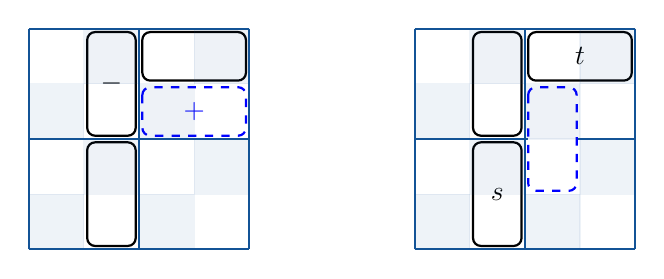
\begin{tikzpicture}[tableau, scale = .7]
              \gridLines{2}{2}
              \verticalDomino{1}{2}{-}
              \horizontalDomino{1}{3}{}
              \horizontalDominoMaybe{2}{3}{+}
              \verticalDomino{3}{2}{}
              \fixedSquaresForGrid{2}{2}

              \gridLinesShift{2}{2}{7}
              \verticalDominoShift{1}{2}{}{7}
              \horizontalDominoShift{1}{3}{t}{7}
              \verticalDominoShift{3}{2}{s}{7}
              \verticalDominoMaybeShift{2}{3}{ }{7}
              \fixedSquaresForGridShift{2}{2}{7}
            \end{tikzpicture}
          \end{figure}
          goes to
          \begin{figure}[H]
            \centering
            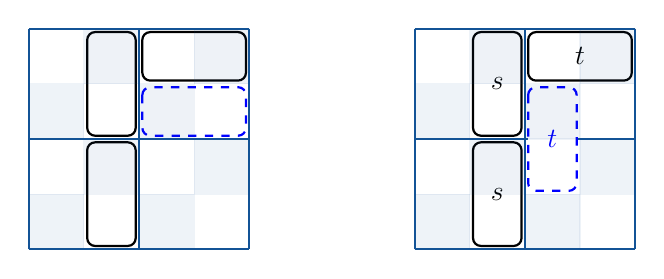
\begin{tikzpicture}[tableau, scale = .7]
              \gridLines{2}{2}
              \verticalDomino{1}{2}{}
              \horizontalDomino{1}{3}{}
              \horizontalDominoMaybe{2}{3}{}
              \verticalDomino{3}{2}{}
              \fixedSquaresForGrid{2}{2}

              \gridLinesShift{2}{2}{7}
              \verticalDominoShift{1}{2}{s}{7}
              \horizontalDominoShift{1}{3}{t}{7}
              \verticalDominoShift{3}{2}{s}{7}
              \verticalDominoMaybeShift{2}{3}{t}{7}
              \fixedSquaresForGridShift{2}{2}{7}
            \end{tikzpicture}
          \end{figure}
          Otherwise, we need to shift the new dominoes and flip their signs on this side.
          \begin{figure}[H]
            \centering
            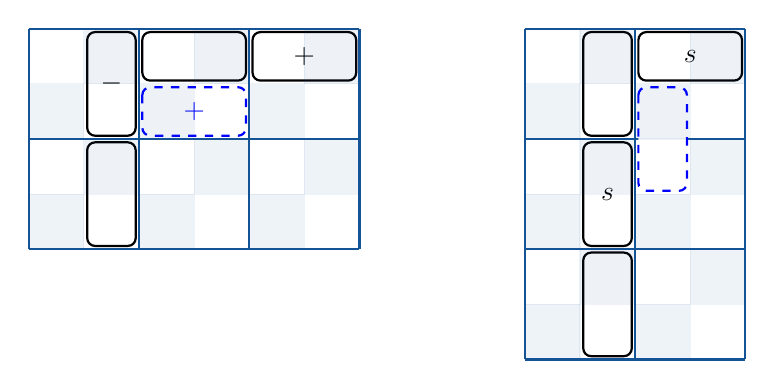
\begin{tikzpicture}[tableau, scale = .7]
              \gridLines{2}{3}
              \verticalDomino{1}{2}{-}
              \horizontalDomino{1}{3}{}
              \horizontalDomino{1}{5}{+}
              \horizontalDominoMaybe{2}{3}{+}
              \verticalDomino{3}{2}{}
              \fixedSquaresForGrid{2}{3}

              \gridLinesShift{3}{2}{9}
              \verticalDominoShift{1}{2}{}{9}
              \horizontalDominoShift{1}{3}{s}{9}
              \verticalDominoShift{3}{2}{s}{9}
              \verticalDominoShift{5}{2}{}{9}
              \verticalDominoMaybeShift{2}{3}{ }{9}
              \fixedSquaresForGridShift{3}{2}{9}
            \end{tikzpicture}
          \end{figure}
          goes to
          \begin{figure}[H]
            \centering
            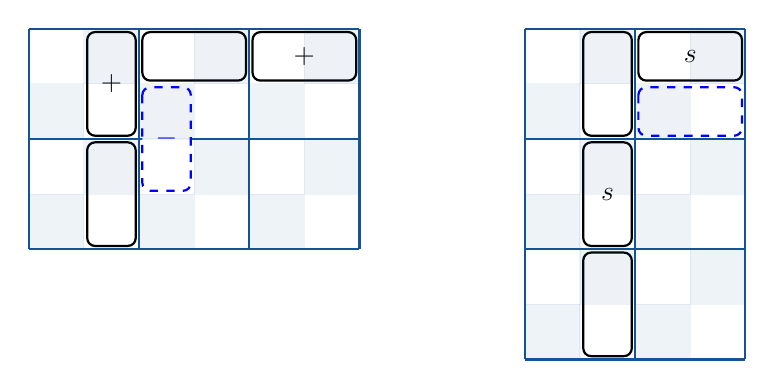
\begin{tikzpicture}[tableau, scale = .7]
              \gridLines{2}{3}
              \verticalDomino{1}{2}{+}
              \horizontalDomino{1}{3}{}
              \horizontalDomino{1}{5}{+}
              \verticalDominoMaybe{2}{3}{-}
              \verticalDomino{3}{2}{}
              \fixedSquaresForGrid{2}{3}

              \gridLinesShift{3}{2}{9}
              \verticalDominoShift{1}{2}{}{9}
              \horizontalDominoShift{1}{3}{s}{9}
              \verticalDominoShift{3}{2}{s}{9}
              \verticalDominoShift{5}{2}{}{9}
              \horizontalDominoMaybeShift{2}{3}{ }{9}
              \fixedSquaresForGridShift{3}{2}{9}
            \end{tikzpicture}
          \end{figure}
          \begin{figure}[H]
            % 1s 2- 3s 4+ 5+
            \centering
            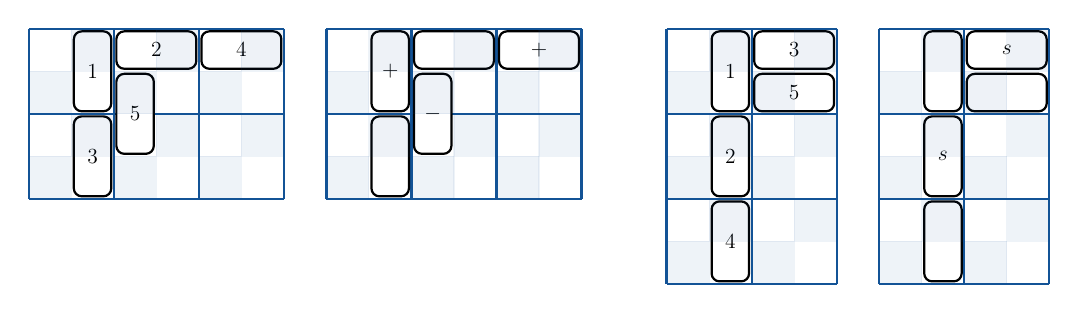
\begin{tikzpicture}[tableau, scale=.54]\gridLines{2}{3}\verticalDomino{1}{2}{1}\horizontalDomino{1}{3}{2}\verticalDomino{3}{2}{3}\horizontalDomino{1}{5}{4}\verticalDomino{2}{3}{5}\fixedSquaresForGrid{2}{3}\gridLinesShift{2}{3}{7}\verticalDominoShift{1}{2}{+}{7}\horizontalDominoShift{1}{3}{}{7}\verticalDominoShift{3}{2}{}{7}\horizontalDominoShift{1}{5}{+}{7}\verticalDominoShift{2}{3}{-}{7}\fixedSquaresForGridShift{2}{3}{7}\gridLinesShift{3}{2}{15}\verticalDominoShift{1}{2}{1}{15}\verticalDominoShift{3}{2}{2}{15}\horizontalDominoShift{1}{3}{3}{15}\verticalDominoShift{5}{2}{4}{15}\horizontalDominoShift{2}{3}{5}{15}\fixedSquaresForGridShift{3}{2}{15}\gridLinesShift{3}{2}{20}\verticalDominoShift{1}{2}{}{20}\verticalDominoShift{3}{2}{s}{20}\horizontalDominoShift{1}{3}{s}{20}\verticalDominoShift{5}{2}{}{20}\horizontalDominoShift{2}{3}{}{20}\fixedSquaresForGridShiftAlt{3}{2}{20}\end{tikzpicture}
          \end{figure}
        \end{itemize}

        Having done this, we notice that a we have created an opportunity for dominoes to move, since the $-$ sign in the pair domino has now been neutralized by the newly-added domino.
        That is, if the rest of the column in the left tableau is blank, and if the bottom of the column is horizontal, there may be a $+$ sign to the left of that bottom domino which can now move into the bottom of the column.
        Concretely speaking, \texttt{switchAfterAddZ()} is called on the dual domino to the blank bottom corner domino.
        Note, moving one domino may make room for another domino to move up.
        The function \texttt{switchAfterAddZ()} calls itself (sometimes) after making the one switch.
        \begin{figure}[H]
          \centering
          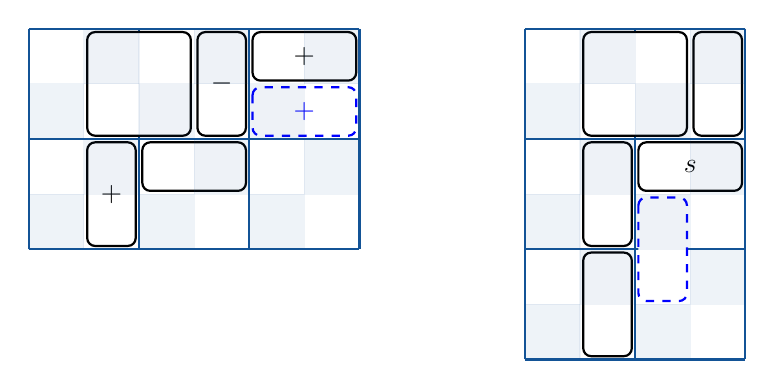
\begin{tikzpicture}[tableau, scale = .7]
            \gridLines{2}{3}
            \emptyBox{1}{2}
            \verticalDomino{1}{4}{-}
            \horizontalDomino{1}{5}{+}
            \horizontalDominoMaybe{2}{5}{+}
            \horizontalDomino{3}{3}{}
            \verticalDomino{3}{2}{+}
            \fixedSquaresForGrid{2}{3}

            \gridLinesShift{3}{2}{9}
            \emptyBoxShift{1}{2}{9}
            \verticalDominoShift{1}{4}{}{9}
            \verticalDominoShift{3}{2}{}{9}
            \horizontalDominoShift{3}{3}{s}{9}
            \verticalDominoShift{5}{2}{}{9}
            \verticalDominoMaybeShift{4}{3}{ }{9}
            \fixedSquaresForGridShift{3}{2}{9}
          \end{tikzpicture}
        \end{figure}
        goes to
        \begin{figure}[H]
          \centering
          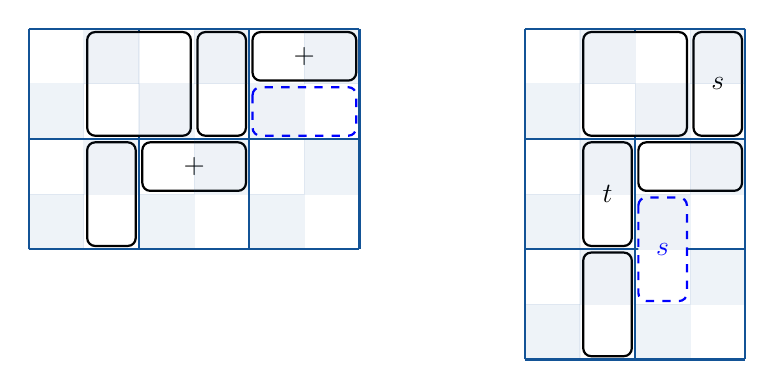
\begin{tikzpicture}[tableau, scale = .7]
            \gridLines{2}{3}
            \emptyBox{1}{2}
            \verticalDomino{1}{4}{}
            \horizontalDomino{1}{5}{+}
            \horizontalDominoMaybe{2}{5}{}
            \horizontalDomino{3}{3}{+}
            \verticalDomino{3}{2}{}
            \fixedSquaresForGrid{2}{3}

            \gridLinesShift{3}{2}{9}
            \emptyBoxShift{1}{2}{9}
            \verticalDominoShift{1}{4}{s}{9}
            \verticalDominoShift{3}{2}{t}{9}
            \horizontalDominoShift{3}{3}{}{9}
            \verticalDominoShift{5}{2}{}{9}
            \verticalDominoMaybeShift{4}{3}{s}{9}
            \fixedSquaresForGridShift{3}{2}{9}
          \end{tikzpicture}
        \end{figure}
        \begin{figure}[H]
          % 2+ 3- 4s 1_5 6+ 7+
          \centering
          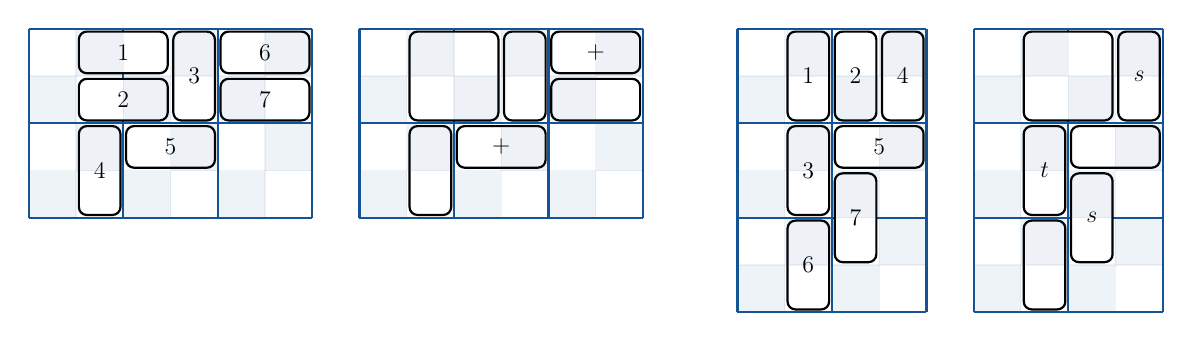
\begin{tikzpicture}[tableau, scale=.6]\gridLines{2}{3}\horizontalDomino{1}{2}{1}\horizontalDomino{2}{2}{2}\verticalDomino{1}{4}{3}\verticalDomino{3}{2}{4}\horizontalDomino{3}{3}{5}\horizontalDomino{1}{5}{6}\horizontalDomino{2}{5}{7}\fixedSquaresForGrid{2}{3}\gridLinesShift{2}{3}{7}\verticalDominoShift{1}{4}{}{7}\verticalDominoShift{3}{2}{}{7}\emptyBoxShift{1}{2}{7}\horizontalDominoShift{3}{3}{+}{7}\horizontalDominoShift{1}{5}{+}{7}\horizontalDominoShift{2}{5}{}{7}\fixedSquaresForGridShift{2}{3}{7}\gridLinesShift{3}{2}{15}\verticalDominoShift{1}{2}{1}{15}\verticalDominoShift{1}{3}{2}{15}\verticalDominoShift{3}{2}{3}{15}\verticalDominoShift{1}{4}{4}{15}\horizontalDominoShift{3}{3}{5}{15}\verticalDominoShift{5}{2}{6}{15}\verticalDominoShift{4}{3}{7}{15}\fixedSquaresForGridShift{3}{2}{15}\gridLinesShift{3}{2}{20}\verticalDominoShift{3}{2}{t}{20}\verticalDominoShift{1}{4}{s}{20}\emptyBoxShift{1}{2}{20}\horizontalDominoShift{3}{3}{}{20}\verticalDominoShift{5}{2}{}{20}\verticalDominoShift{4}{3}{s}{20}\fixedSquaresForGridShiftAlt{3}{2}{20}\end{tikzpicture}
        \end{figure}
        \item Here the pair domino is blank.
        There are a number of cases.
        In them we have a top domino, which is above the domino which we are tryng to add, and a side domino, which is directly below the pair domino.
        We also have these on the dual side, that is, the dual top domino corresponds to the side domino, and the dual side domino corresponds to the top domino.
        \begin{itemize}
          \item Here the top domino contains $-$.
          Then we are basically good to go.
          We'll blank the top signs and fill them on the dual side.
          First, we'll call \texttt{prepareForSign()} on the dual side, so as to be able to place a sign in the dual side domino.
          \begin{figure}[H]
            \centering
            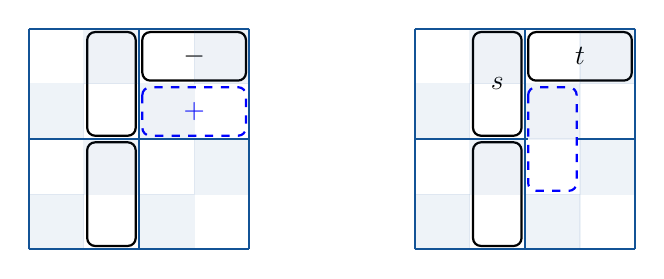
\begin{tikzpicture}[tableau, scale = .7]
              \gridLines{2}{2}
              \verticalDomino{1}{2}{}
              \horizontalDomino{1}{3}{-}
              \horizontalDominoMaybe{2}{3}{+}
              \verticalDomino{3}{2}{}
              \fixedSquaresForGrid{2}{2}

              \gridLinesShift{2}{2}{7}
              \verticalDominoShift{1}{2}{s}{7}
              \horizontalDominoShift{1}{3}{t}{7}
              \verticalDominoShift{3}{2}{}{7}
              \verticalDominoMaybeShift{2}{3}{ }{7}
              \fixedSquaresForGridShift{2}{2}{7}
            \end{tikzpicture}
          \end{figure}
          \noindent goes to
          \begin{figure}[H]
            \centering
            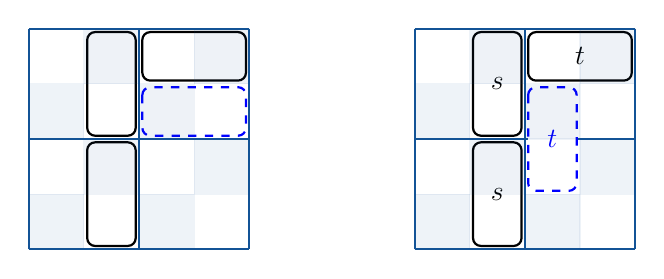
\begin{tikzpicture}[tableau, scale = .7]
              \gridLines{2}{2}
              \verticalDomino{1}{2}{}
              \horizontalDomino{1}{3}{}
              \horizontalDominoMaybe{2}{3}{}
              \verticalDomino{3}{2}{}
              \fixedSquaresForGrid{2}{2}

              \gridLinesShift{2}{2}{7}
              \verticalDominoShift{1}{2}{s}{7}
              \horizontalDominoShift{1}{3}{t}{7}
              \verticalDominoShift{3}{2}{s}{7}
              \verticalDominoMaybeShift{2}{3}{t}{7}
              \fixedSquaresForGridShift{2}{2}{7}
            \end{tikzpicture}
          \end{figure}
          \begin{figure}[H]
            % 1s 2t 3_4
            \centering
            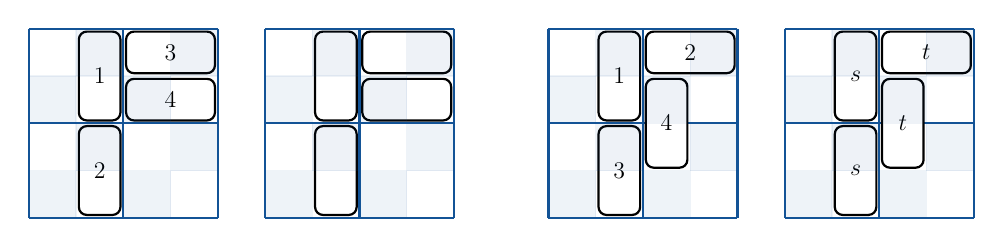
\begin{tikzpicture}[tableau, scale=.6]\gridLines{2}{2}\verticalDomino{1}{2}{1}\verticalDomino{3}{2}{2}\horizontalDomino{1}{3}{3}\horizontalDomino{2}{3}{4}\fixedSquaresForGrid{2}{2}\gridLinesShift{2}{2}{5}\verticalDominoShift{1}{2}{}{5}\verticalDominoShift{3}{2}{}{5}\horizontalDominoShift{1}{3}{}{5}\horizontalDominoShift{2}{3}{}{5}\fixedSquaresForGridShift{2}{2}{5}\gridLinesShift{2}{2}{11}\verticalDominoShift{1}{2}{1}{11}\horizontalDominoShift{1}{3}{2}{11}\verticalDominoShift{3}{2}{3}{11}\verticalDominoShift{2}{3}{4}{11}\fixedSquaresForGridShift{2}{2}{11}\gridLinesShift{2}{2}{16}\verticalDominoShift{1}{2}{s}{16}\horizontalDominoShift{1}{3}{t}{16}\verticalDominoShift{3}{2}{s}{16}\verticalDominoShift{2}{3}{t}{16}\fixedSquaresForGridShiftAlt{2}{2}{16}\end{tikzpicture}
          \end{figure}
          \noindent Or, starting with one more $+$ domino in the top row, we get
          \begin{figure}[H]
            % 1s 2t 3- 4+ 5+
            \centering
            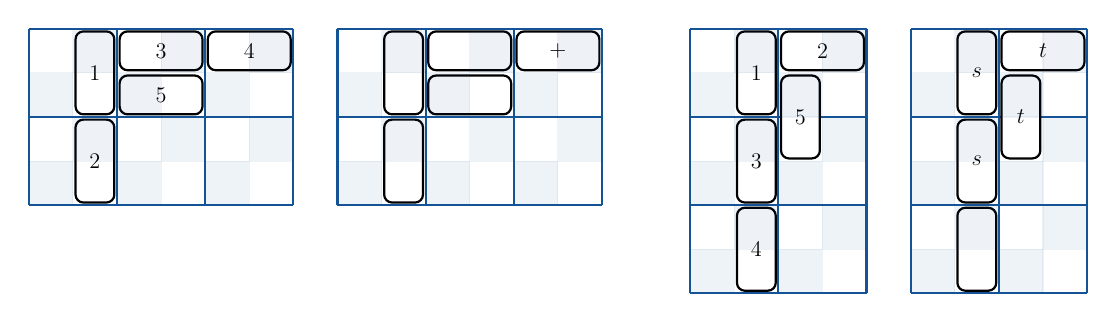
\begin{tikzpicture}[tableau, scale=.56]\gridLines{2}{3}\verticalDomino{1}{2}{1}\verticalDomino{3}{2}{2}\horizontalDomino{1}{3}{3}\horizontalDomino{1}{5}{4}\horizontalDomino{2}{3}{5}\fixedSquaresForGrid{2}{3}\gridLinesShift{2}{3}{7}\verticalDominoShift{1}{2}{}{7}\verticalDominoShift{3}{2}{}{7}\horizontalDominoShift{1}{3}{}{7}\horizontalDominoShift{1}{5}{+}{7}\horizontalDominoShift{2}{3}{}{7}\fixedSquaresForGridShift{2}{3}{7}\gridLinesShift{3}{2}{15}\verticalDominoShift{1}{2}{1}{15}\horizontalDominoShift{1}{3}{2}{15}\verticalDominoShift{3}{2}{3}{15}\verticalDominoShift{5}{2}{4}{15}\verticalDominoShift{2}{3}{5}{15}\fixedSquaresForGridShift{3}{2}{15}\gridLinesShift{3}{2}{20}\verticalDominoShift{1}{2}{s}{20}\horizontalDominoShift{1}{3}{t}{20}\verticalDominoShift{3}{2}{s}{20}\verticalDominoShift{5}{2}{}{20}\verticalDominoShift{2}{3}{t}{20}\fixedSquaresForGridShiftAlt{3}{2}{20}\end{tikzpicture}
          \end{figure}
          \item Here the top domino contains $+$.
          (Note, in the code, this is the third case.)
          \begin{figure}[H]
            \centering
            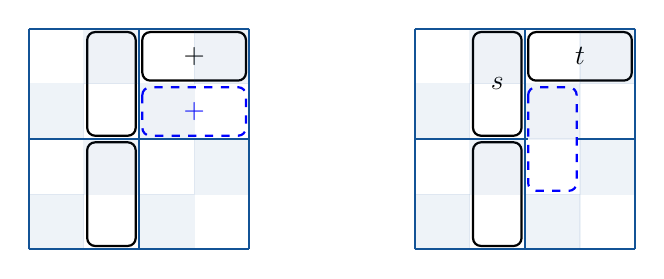
\begin{tikzpicture}[tableau, scale = .7]
              \gridLines{2}{2}
              \verticalDomino{1}{2}{}
              \horizontalDomino{1}{3}{+}
              \horizontalDominoMaybe{2}{3}{+}
              \verticalDomino{3}{2}{}
              \fixedSquaresForGrid{2}{2}

              \gridLinesShift{2}{2}{7}
              \verticalDominoShift{1}{2}{s}{7}
              \horizontalDominoShift{1}{3}{t}{7}
              \verticalDominoShift{3}{2}{}{7}
              \verticalDominoMaybeShift{2}{3}{ }{7}
              \fixedSquaresForGridShift{2}{2}{7}
            \end{tikzpicture}
          \end{figure}
          goes to
          \begin{figure}[H]
            \centering
            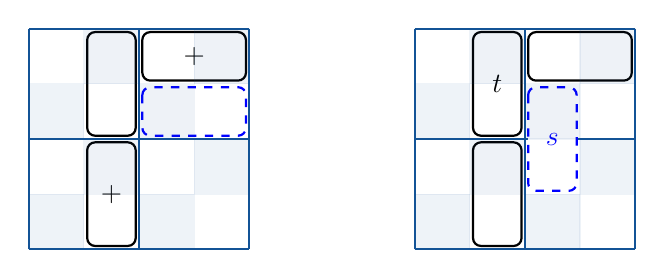
\begin{tikzpicture}[tableau, scale = .7]
              \gridLines{2}{2}
              \verticalDomino{1}{2}{}
              \horizontalDomino{1}{3}{+}
              \horizontalDominoMaybe{2}{3}{}
              \verticalDomino{3}{2}{+}
              \fixedSquaresForGrid{2}{2}

              \gridLinesShift{2}{2}{7}
              \verticalDominoShift{1}{2}{t}{7}
              \horizontalDominoShift{1}{3}{}{7}
              \verticalDominoShift{3}{2}{}{7}
              \verticalDominoMaybeShift{2}{3}{s}{7}
              \fixedSquaresForGridShift{2}{2}{7}
            \end{tikzpicture}
          \end{figure}
          \begin{figure}[H]
            % 1s 2t 3+ 4+
            \centering
            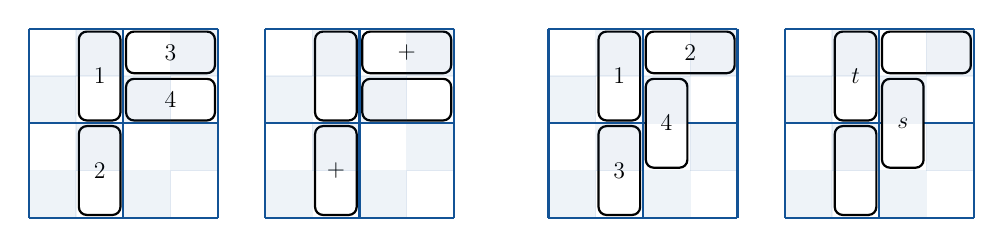
\begin{tikzpicture}[tableau, scale=.6]\gridLines{2}{2}\verticalDomino{1}{2}{1}\verticalDomino{3}{2}{2}\horizontalDomino{1}{3}{3}\horizontalDomino{2}{3}{4}\fixedSquaresForGrid{2}{2}\gridLinesShift{2}{2}{5}\verticalDominoShift{1}{2}{}{5}\verticalDominoShift{3}{2}{+}{5}\horizontalDominoShift{1}{3}{+}{5}\horizontalDominoShift{2}{3}{}{5}\fixedSquaresForGridShift{2}{2}{5}\gridLinesShift{2}{2}{11}\verticalDominoShift{1}{2}{1}{11}\horizontalDominoShift{1}{3}{2}{11}\verticalDominoShift{3}{2}{3}{11}\verticalDominoShift{2}{3}{4}{11}\fixedSquaresForGridShift{2}{2}{11}\gridLinesShift{2}{2}{16}\verticalDominoShift{1}{2}{t}{16}\horizontalDominoShift{1}{3}{}{16}\verticalDominoShift{3}{2}{}{16}\verticalDominoShift{2}{3}{s}{16}\fixedSquaresForGridShiftAlt{2}{2}{16}\end{tikzpicture}
          \end{figure}
          \item Here the top domino is blank.
          (Note, in the code, this is the second case.)
          We need to find the sign in the top row.
          (TODO, there must be a sign in the top row.  Why?)
          There are two cases.

          Here the sign in the top row is $-$. This is basically the same as the situation where the top domino is $-$.
          \begin{figure}[H]
            \centering
            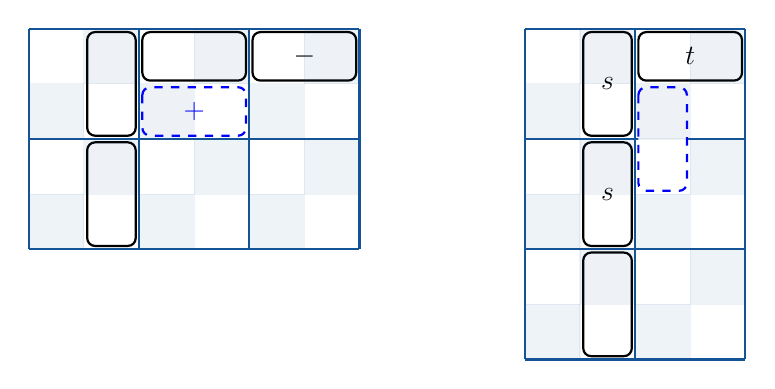
\begin{tikzpicture}[tableau, scale = .7]
              \gridLines{2}{3}
              \verticalDomino{1}{2}{}
              \horizontalDomino{1}{3}{}
              \horizontalDomino{1}{5}{-}
              \horizontalDominoMaybe{2}{3}{+}
              \verticalDomino{3}{2}{}
              \fixedSquaresForGrid{2}{3}

              \gridLinesShift{3}{2}{9}
              \verticalDominoShift{1}{2}{s}{9}
              \horizontalDominoShift{1}{3}{t}{9}
              \verticalDominoShift{3}{2}{s}{9}
              \verticalDominoShift{5}{2}{}{9}
              \verticalDominoMaybeShift{2}{3}{ }{9}
              \fixedSquaresForGridShift{3}{2}{9}
            \end{tikzpicture}
          \end{figure}
          \noindent goes to
          \begin{figure}[H]
            \centering
            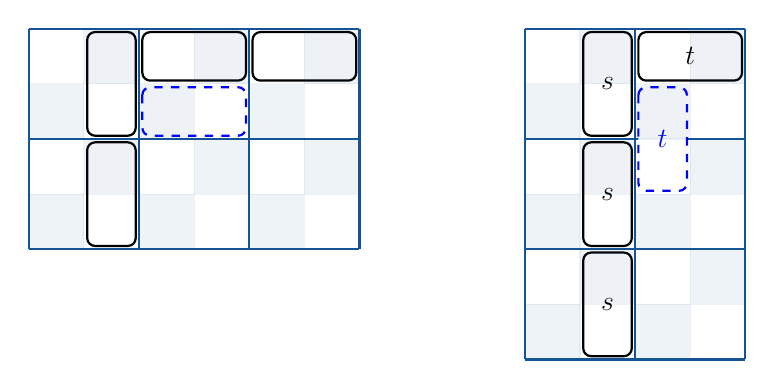
\begin{tikzpicture}[tableau, scale = .7]
              \gridLines{2}{3}
              \verticalDomino{1}{2}{}
              \horizontalDomino{1}{3}{}
              \horizontalDomino{1}{5}{}
              \horizontalDominoMaybe{2}{3}{}
              \verticalDomino{3}{2}{}
              \fixedSquaresForGrid{2}{3}

              \gridLinesShift{3}{2}{9}
              \verticalDominoShift{1}{2}{s}{9}
              \horizontalDominoShift{1}{3}{t}{9}
              \verticalDominoShift{3}{2}{s}{9}
              \verticalDominoShift{5}{2}{s}{9}
              \verticalDominoMaybeShift{2}{3}{t}{9}
              \fixedSquaresForGridShift{3}{2}{9}
            \end{tikzpicture}
          \end{figure}
          \begin{figure}[H]
            % 1s 2s 3t 4_5
            \centering
            \begin{tikzpicture}[tableau, scale=.56]\gridLines{2}{3}\verticalDomino{1}{2}{1}\horizontalDomino{1}{3}{2}\verticalDomino{3}{2}{3}\horizontalDomino{1}{5}{4}\horizontalDomino{2}{3}{5}\fixedSquaresForGrid{2}{3}\gridLinesShift{2}{3}{7}\verticalDominoShift{1}{2}{}{7}\horizontalDominoShift{1}{3}{}{7}\verticalDominoShift{3}{2}{}{7}\horizontalDominoShift{1}{5}{}{7}\horizontalDominoShift{2}{3}{}{7}\fixedSquaresForGridShift{2}{3}{7}\gridLinesShift{3}{2}{15}\verticalDominoShift{1}{2}{1}{15}\verticalDominoShift{3}{2}{2}{15}\horizontalDominoShift{1}{3}{3}{15}\verticalDominoShift{5}{2}{4}{15}\verticalDominoShift{2}{3}{5}{15}\fixedSquaresForGridShift{3}{2}{15}\gridLinesShift{3}{2}{20}\verticalDominoShift{1}{2}{s}{20}\verticalDominoShift{3}{2}{s}{20}\horizontalDominoShift{1}{3}{t}{20}\verticalDominoShift{5}{2}{s}{20}\verticalDominoShift{2}{3}{t}{20}\fixedSquaresForGridShiftAlt{3}{2}{20}\end{tikzpicture}
          \end{figure}
          \noindent Or, with an extra $+$ domino in the top row,
          \begin{figure}[H]
            % 1s 2s 3t 4- 5+ 6+
            \centering
            \begin{tikzpicture}[tableau, scale=.48]\gridLines{2}{4}\verticalDomino{1}{2}{1}\horizontalDomino{1}{3}{2}\verticalDomino{3}{2}{3}\horizontalDomino{1}{5}{4}\horizontalDomino{1}{7}{5}\horizontalDomino{2}{3}{6}\fixedSquaresForGrid{2}{4}\gridLinesShift{2}{4}{9}\verticalDominoShift{1}{2}{}{9}\horizontalDominoShift{1}{3}{}{9}\verticalDominoShift{3}{2}{}{9}\horizontalDominoShift{1}{5}{}{9}\horizontalDominoShift{1}{7}{+}{9}\horizontalDominoShift{2}{3}{}{9}\fixedSquaresForGridShift{2}{4}{9}\gridLinesShift{4}{2}{19}\verticalDominoShift{1}{2}{1}{19}\verticalDominoShift{3}{2}{2}{19}\horizontalDominoShift{1}{3}{3}{19}\verticalDominoShift{5}{2}{4}{19}\verticalDominoShift{7}{2}{5}{19}\verticalDominoShift{2}{3}{6}{19}\fixedSquaresForGridShift{4}{2}{19}\gridLinesShift{4}{2}{24}\verticalDominoShift{1}{2}{s}{24}\verticalDominoShift{3}{2}{s}{24}\horizontalDominoShift{1}{3}{t}{24}\verticalDominoShift{5}{2}{s}{24}\verticalDominoShift{7}{2}{}{24}\verticalDominoShift{2}{3}{t}{24}\fixedSquaresForGridShiftAlt{4}{2}{24}\end{tikzpicture}
          \end{figure}
          Here the sign in the top row is $+$.
          \begin{figure}[H]
            \centering
            \begin{tikzpicture}[tableau, scale = .7]
              \gridLines{2}{3}
              \verticalDomino{1}{2}{}
              \horizontalDomino{1}{3}{}
              \horizontalDomino{1}{5}{+}
              \horizontalDominoMaybe{2}{3}{+}
              \verticalDomino{3}{2}{}
              \fixedSquaresForGrid{2}{3}

              \gridLinesShift{3}{2}{9}
              \verticalDominoShift{1}{2}{s}{9}
              \horizontalDominoShift{1}{3}{t}{9}
              \verticalDominoShift{3}{2}{s}{9}
              \verticalDominoShift{5}{2}{}{9}
              \verticalDominoMaybeShift{2}{3}{ }{9}
              \fixedSquaresForGridShift{3}{2}{9}
            \end{tikzpicture}
          \end{figure}
          goes to
          \begin{figure}[H]
            \centering
            \begin{tikzpicture}[tableau, scale = .7]
              \gridLines{2}{3}
              \verticalDomino{1}{2}{+}
              \horizontalDomino{1}{3}{}
              \horizontalDomino{1}{5}{+}
              \verticalDominoMaybe{2}{3}{-}
              \verticalDomino{3}{2}{+}
              \fixedSquaresForGrid{2}{3}

              \gridLinesShift{3}{2}{9}
              \verticalDominoShift{1}{2}{}{9}
              \horizontalDominoShift{1}{3}{}{9}
              \verticalDominoShift{3}{2}{s}{9}
              \verticalDominoShift{5}{2}{}{9}
              \horizontalDominoMaybeShift{2}{3}{ }{9}
              \fixedSquaresForGridShift{3}{2}{9}
            \end{tikzpicture}
          \end{figure}
          \begin{figure}[H]
            % 1s 2s 3t 4+ 5+
            \centering
            \begin{tikzpicture}[tableau, scale=.56]\gridLines{2}{3}\verticalDomino{1}{2}{1}\horizontalDomino{1}{3}{2}\verticalDomino{3}{2}{3}\horizontalDomino{1}{5}{4}\verticalDomino{2}{3}{5}\fixedSquaresForGrid{2}{3}\gridLinesShift{2}{3}{7}\verticalDominoShift{1}{2}{+}{7}\horizontalDominoShift{1}{3}{}{7}\verticalDominoShift{3}{2}{+}{7}\horizontalDominoShift{1}{5}{+}{7}\verticalDominoShift{2}{3}{-}{7}\fixedSquaresForGridShift{2}{3}{7}\gridLinesShift{3}{2}{15}\verticalDominoShift{1}{2}{1}{15}\verticalDominoShift{3}{2}{2}{15}\horizontalDominoShift{1}{3}{3}{15}\verticalDominoShift{5}{2}{4}{15}\horizontalDominoShift{2}{3}{5}{15}\fixedSquaresForGridShift{3}{2}{15}\gridLinesShift{3}{2}{20}\verticalDominoShift{1}{2}{}{20}\verticalDominoShift{3}{2}{s}{20}\horizontalDominoShift{1}{3}{}{20}\verticalDominoShift{5}{2}{}{20}\horizontalDominoShift{2}{3}{}{20}\fixedSquaresForGridShiftAlt{3}{2}{20}\end{tikzpicture}
          \end{figure}
          So, how do we think about this outcome?
          We can think that this is related to the outcome when $+$ is in the top domino.
          That is, if we interchange the two top dominoes, then, seeing two $+$ dominoes together, the cycle would respond by moving up.
          It would look like this.
          \begin{figure}[H]
            \centering
            \begin{tikzpicture}[tableau, scale = .7]
              \gridLines{2}{3}
              \verticalDomino{1}{2}{}
              \horizontalDomino{1}{3}{+}
              \horizontalDomino{1}{5}{}
              \horizontalDomino{2}{3}{}
              \verticalDomino{3}{2}{+}
              \fixedSquaresForGrid{2}{3}

              \gridLinesShift{3}{2}{9}
              \verticalDominoShift{1}{2}{t}{9}
              \horizontalDominoShift{1}{3}{}{9}
              \verticalDominoShift{3}{2}{}{9}
              \verticalDominoShift{5}{2}{s}{9}
              \verticalDominoShift{2}{3}{s}{9}
              \fixedSquaresForGridShift{3}{2}{9}
            \end{tikzpicture}
          \end{figure}
          It also might help to look at the input which leads to the conjugate result, that is, with the cycle up.
          It's this:
          \begin{figure}[H]
            % 1+ 2- 3s 4+
            \centering
            \begin{tikzpicture}[tableau, scale=.56]\gridLines{2}{3}\verticalDomino{1}{2}{1}\horizontalDomino{1}{3}{2}\verticalDomino{3}{2}{3}\horizontalDomino{1}{5}{4}\fixedSquaresForGrid{2}{3}\gridLinesShift{2}{3}{7}\verticalDominoShift{1}{2}{+}{7}\horizontalDominoShift{1}{3}{-}{7}\verticalDominoShift{3}{2}{}{7}\horizontalDominoShift{1}{5}{+}{7}\fixedSquaresForGridShift{2}{3}{7}\gridLinesShift{3}{2}{15}\verticalDominoShift{1}{2}{1}{15}\verticalDominoShift{3}{2}{2}{15}\horizontalDominoShift{1}{3}{3}{15}\verticalDominoShift{5}{2}{4}{15}\fixedSquaresForGridShift{3}{2}{15}\gridLinesShift{3}{2}{20}\verticalDominoShift{1}{2}{}{20}\verticalDominoShift{3}{2}{}{20}\horizontalDominoShift{1}{3}{s}{20}\verticalDominoShift{5}{2}{}{20}\fixedSquaresForGridShiftAlt{3}{2}{20}\end{tikzpicture}
          \end{figure}
          goes to
          \begin{figure}[H]
            % 1+ 2- 3s 4+ 5+
            \centering
            \begin{tikzpicture}[tableau, scale=.56]\gridLines{2}{3}\verticalDomino{1}{2}{1}\horizontalDomino{1}{3}{2}\verticalDomino{3}{2}{3}\horizontalDomino{1}{5}{4}\horizontalDomino{2}{3}{5}\fixedSquaresForGrid{2}{3}\gridLinesShift{2}{3}{7}\verticalDominoShift{1}{2}{}{7}\horizontalDominoShift{1}{3}{}{7}\verticalDominoShift{3}{2}{+}{7}\horizontalDominoShift{1}{5}{+}{7}\horizontalDominoShift{2}{3}{}{7}\fixedSquaresForGridShift{2}{3}{7}\gridLinesShift{3}{2}{15}\verticalDominoShift{1}{2}{1}{15}\verticalDominoShift{3}{2}{2}{15}\horizontalDominoShift{1}{3}{3}{15}\verticalDominoShift{5}{2}{4}{15}\verticalDominoShift{2}{3}{5}{15}\fixedSquaresForGridShift{3}{2}{15}\gridLinesShift{3}{2}{20}\verticalDominoShift{1}{2}{s}{20}\verticalDominoShift{3}{2}{s}{20}\horizontalDominoShift{1}{3}{}{20}\verticalDominoShift{5}{2}{}{20}\verticalDominoShift{2}{3}{t}{20}\fixedSquaresForGridShiftAlt{3}{2}{20}\end{tikzpicture}
          \end{figure}
        \end{itemize}
        To conclude the discussion of the case where the pair domino is vertical and blank, we note that,
        as in the case when the pair domino is vertical and has a minus sign, there may now be an opportunity for a domino to move.
        This time, we have that an $s$ (or $t$) in the pair domino on the dual side has been neutralized.
        So, we may call \texttt{switchAfterAddZ()} on this side.
      \end{itemize}
    \end{itemize}
  \end{itemize}
\end{document}
